\documentclass[a4paper]{article}
\usepackage[german]{babel}
\usepackage[utf8]{inputenc}
\usepackage{amsmath}
\usepackage{amsfonts} 
% package for including graphics with figure-environment
\usepackage{graphicx}
\usepackage{hyperref}
\usepackage{float}
\usepackage{amssymb,stmaryrd}
% colors for hyperlinks
\hypersetup{colorlinks=true,citecolor=black,filecolor=black,linkcolor=black,urlcolor=black}

% Commentbox package
\usepackage[most]{tcolorbox}
% Braket notation package
\usepackage{braket}

% Commentbox package
% package for header
\usepackage[automark,headsepline]{scrlayer-scrpage}
\usepackage[T1]{fontenc}
\usepackage{color}
\usepackage{mathtools}
\usepackage{comment}



\pagestyle{scrheadings}
\ihead[]{Meyer, Springer, Kawamura, Heidenreich}
\ohead[]{\today}
\cfoot[]{\pagemark}

\begin{document}
	\title{
	\begin{figure}[!ht]
		% \flushleft
			
\includegraphics[width=0.26\textwidth]{img/THlogoheader.pdf}
	\end{figure}
	\vspace{1cm}
	\Huge Quantencomputer Verstehen
	}
	
	\vspace{1cm}
	
	% if you are the only author, you might use the following
	% \author{Name of student}	
	
	% Insert here your name and correct mail address
	\author{\Large \href{mailto:ben_konrad.meyer@smail.th-koeln.de@smail.th-koeln.de}{Ben Konrad Meyer} \and \Large \href{mailto:mike.springer@smail.th-koeln.de}{Mike Springer} \and \Large \href{mailto:kai.kawamura@smail.th-koeln.de}{Kai Kawamura} \and \Large \href{mailto:karl_julian.heidenreich@smail.th-koeln.de}{Julian Heidenreich} \\
	\vspace{1cm}}
	
	% name of the course and module
	\date{
	\large Modul: Verteilte Systeme \\ 
	\vspace{0.8cm}
	\large Dozent: Lutz Köhler \\
	\vspace{1cm}
	\today
	}

	\maketitle
	\setlength{\parindent}{0pt}

\vspace{2cm}
	\newpage
	\tableofcontents
	\newpage
	
\section{Einleitung}
\label{sec:einleitung}

Die Quanteninformatik ist ein schnell wachsendes Forschungsfeld. \footnote{\cite[S. XII.]{homeister_quantum_2022}}
Anders als klassische Computer, die auf Bits basieren und nur die Zustände 0 und 1 kennen, nutzt die Quanteninformatik sogenannte Quantenbits (Qubits), die in einer Superposition beide Zustände gleichzeitig annehmen können.
Dies führt zu einer völlig neuen Art der Datenverarbeitung, die in vielen Bereichen eine deutlich höhere Effizienz verspricht und potenziell über die Fähigkeiten heutiger Computersysteme hinausgeht.\\

In den letzten Jahren wurde vielversprechende Forschung zu verschiedenen Aspekten der Quanteninformatik durchgeführt, wie der Implementierung von Quantenalgorithmen, der Nutzung von Verschränkung und der Fehlertoleranz in Quantencomputern.
Diese Entwicklungen eröffnen neue Möglichkeiten unter anderem in Bereichen wie Kryptografie, Simulation chemischer Reaktionen und maschinelles Lernen.\footnote{\cite{Fraunhofer_quantencomputing_2025}}\\

In dieser Arbeit werden wir die Grundlagen der Quanteninformatik erläutern und einige der wichtigsten Konzepte und Prinzipien vorstellen.
Wir beginnen mit einer Einführung und erklären in welchen Bereichen sich ein Quantencomputer von einem klassischen Computer unterscheidet.
Dazu gehören Quantenbits und die Superposition, sowie Quantenregister und die Funktion der Verschränkung.
Außerdem werden wir die Bedeutung von Quantengattern und Quantenschaltkreisen erläutern und einen kurzen Umriss der uns jetzt schon bekannten Grenzen sowie zukünftiger Anwendungsgebiete geben.
Nach den Grundlagen kommen wir zu weiterführenden Themen, wie dem No Cloning Theorem und der Quantenteleportation.
Wie funktioniert die Quantenteleportation und was sind Herausforderungen?
Als letztes Thema werden wir uns mit der Quantenhardware beschäftigen, mit besonderem Fokus auf universellen Quantencomputern und der Error Correction.
\section{Einführung in die Quanteninformatik} 
\label{sec:Einführung in die Quanteninformatik}
\subsection{Quantenbits}
Ein Quantenbit, im Folgenden auch Qubit genannt, ist das Medium und die kleinste Einheit, auf dem in der Quanteninformatik gerechnet wird. Auf die genaue physische Realisierung wird in einem späteren Abschnitt der Quantenhardware eingegangen. Bis dahin reicht es das Quantenbit als eine Art Computer-Bit zu verstehen, das sich in einer sogenannten ``Superposition'' befindet. Im Zustand der Superposition kann es gleichzeitig den Wert ‚0‘ und ‚1‘ annehmen. Ein Quantenbit bleibt in dieser Superposition, bis es gemessen wird, woraufhin die Superposition zerstört wird und das Qubit einen der Zustände 0 oder 1 annimmt. Die Wahrscheinlichkeit, mit der ein Quantenbit in den einen oder anderen Zustand zerfällt, muss nicht gleich verteilt sein und kann beeinflusst werden. Dies macht Berechnungen auf Qubits erst möglich.\\

Mathematisch betrachtet, werden die Zustände ‚0‘ und ‚1‘ in der Quanteninformatik als Vektoren \(\binom{1}{0}\) $\equiv$ 0 und \(\binom{0}{1}\) $\equiv$ 1 dargestellt. Für die einfache Lesbarkeit werden diese Vektoren in der Quanteninformatik in der Bra-Ket-Notation dargestellt.
Also \(\binom{1}{0}\) $\equiv$ $\left|0\right\rangle$ und \(\binom{0}{1}\) $\equiv$ $\left|1\right\rangle$. \\

Um die Wahrscheinlichkeit zu beschreiben, welchen der beiden Werte ein Quantenbit nach der Messung annimmt, werden beiden Werten eine Amplitude $\alpha$ oder $\beta$ zugeordnet. Demnach wird ein Quantenbit in einer beliebigen Superposition als $\alpha\cdot\left|0\right\rangle+\beta\cdot\left|1\right\rangle$ dargestellt. $\alpha$ und $\beta$ sind komplexe Zahlen für die $\left|\alpha\right|^2+\left|\beta\right|^2=1$ gilt. 

Ein Qbit, das nach der Messung mit gleicher Wahrscheinlichkeit in einen der beiden Zustände 0 und 1 zerfällt, würde folglich als $\frac{1}{\sqrt2}\cdot\left|0\right\rangle+\frac{1}{\sqrt2}\cdot\left|1\right\rangle$ oder $\frac{1}{\sqrt{2}}(\left|0\right.\rangle+\left|1\right.\rangle)$ dargestellt werden. Dabei gilt $\alpha = \beta = \frac{1}{\sqrt2}$ und erfüllt die Bedingung $\left|\frac{1}{\sqrt2}\right|^2+\left|\frac{1}{\sqrt2}\right|^2=1$.\\

Ein Vektor $\binom{\alpha}{\beta}$ wird als ``
Zustandsvektor'' bezeichnet und stellt den Zustand der Superposition eines Qubits dar. Die Bedingung $\left|\alpha\right|^2+\left|\beta\right|^2=1$ sorgt dafür, dass der Zustandsvektor immer ein Einheitsvektor ist. Dadurch kann jeder Zustand eines Qubits auf dem Einheitskreis eines zweidimensionalen Vektorsystems dargestellt werden. Somit kann ein Quantenbit unendlich viele Zustände haben, die auf einen definierten Bereich abgebildet werden können. 

\begin{tcolorbox}[title=Kommentar,
    title filled=false,
    colback=cyan!5!white,
    colframe=cyan!75!black]
Zu dem Zeitpunkt, als wir uns das Grundwissen erarbeitet haben, war uns nicht klar, weshalb $\alpha$ und $\beta$ komplexe Zahlen sein müssten und warum sie „Amplituden“ und nicht „Wahrscheinlichkeiten“ oder Ähnliches genannt werden. Wir gingen davon aus, dass wir früher oder später auf einen Use Case stoßen würden, in denen komplexe Zahlen und Amplituden wichtig werden. Dies war allerdings nur für letztes bedingt der Fall. Um kurz vorzugreifen: Amplituden von zwei Qubits können miteinander summiert werden. Dadurch ist es möglich, dass sich manche Amplituden gegenseitig aufheben. Dies wäre mit Wahrscheinlichkeitsverteilungen, die nicht negativ sein dürften, schwer darzustellen\footnote{\cite{homeister_quantum_2022}}.

Warum $\alpha$ und $\beta$ komplexe Zahlen sind, war schwer greifbar. Scheinbar hat dies mit der der Quanteninformatik zugrundeliegenden Quantenmechanik zu tun. Nach etwas Recherchearbeit stellte sich heraus, dass eine Antwort auf diese Frage einiges an Vorwissen in der Physik bedurfte. Da wir uns diese Frage am Anfang des Lernprozesses stellten und noch dabei waren in den Konzepten der Quanteninformatik Fuß fassen, entscheiden wir uns auf diese Frage zurück zu kommen, sobald komplexe Zahlen relevant werden würden. Da in der Quanteninformatik mit $\alpha$ und $\beta$ allerdings gerechnet wird, als seien sie reelle Zahlen\footnote{\cite{why_complex_numbers}} und nur für die Umstellung der Formeln die Rechenregeln für komplexe Zahlen genutzt werden\footnote{\cite{homeister_quantum_2022}}, trat dieser Fall nie wirklich ein.

Während der Erstellung dieses Dokuments haben uns unsere erlangten Kenntnisse beim Verstehen der Quantenmechanik nicht sonderlich weiter helfen können, um eine zufriedenstellende Antwort zu formulieren. Da es sehr zeitaufwändig geworden wäre, sämtliche Begrifflichkeiten wie aus dem Kurs Skript von John D Stack\footnote{\cite{no_title}} zu verstehen, nur um diese Frage zu klären, entscheiden wir uns dieser nicht weiter nachzugehen. Das, was wir uns zusammen reimen konnten, ist, dass der Zustand von Partikeln in der Quantenmechanik als Wellenfunktion dargestellt wird. Um mit diesen rechnen zu können, ist der Imaginärteil der komplexen Zahlen notwendig. Es wäre sicherlich hilfreich gewesen die quantenmechanischen Hintergründe zu verstehen, bevor wir uns mit der Quanteninformatik auseinander gesetzt haben, allerdings hätte dies den Rahmen unseres Themas deutlich gesprengt.
\end{tcolorbox}

Um mit Quantenbits rechnen zu können, muss man den Zustand eines Quantenbits verändern können. Wie dies technisch umgesetzt wird, wird später angerissen. Aus mathematischer Sicht geschieht dies über unitäre $2\times2$ Matrizen. \\

Eine Matrix A ist dann unitär, wenn ihre inverse Matrix $A^{-1}$ gleich ihrer adjungierten Matrix $A^\dag$ ist. Adjungiert ist eine Matrix $A^\dag$ dann, wenn die Matrix A komplex konjugiert – also jedes Element der Matrix $z_{ij}=a+ib$ zu $z_{ij}^\ast=a-ib$ komplex konjugiert – und die Matrix dann transponiert wird. Also muss für alle Matritzen A gelten:
\begin{equation}
    A^{-1}=(A^*)^T=A^\dag
\end{equation}

Für die Quanteninformatik reicht oft die Bedingung $A^{-1}=A^T$, da hier meist mit $\alpha$ und $\beta$ gerechnet wird, als seien sie reelle Zahlen. Durch diese Bedingung haben unitäre Matrizen die Eigenschaft, dass ein Zustandsvektor unverändert bleibt, wenn eine unitäre Matrix zwei Mal mit ihm verrechnet wird. 

Unitäre Transformationen sind also reversibel. Diese Bedingung ist notwendig, um die Länge der Zustandsvektoren beizubehalten.

Beispielhaft kann dies an einer Matrix 
\begin{equation}
    B=\left(\begin{matrix}\frac{1}{2}&\frac{\sqrt3}{2}\\\frac{\sqrt3}{2}&-\frac{1}{2}\\\end{matrix}\right)
\end{equation} demonstriert werden. Wendet man diese Matrix auf ein Qubit im Zustand $\left|0\right\rangle$ an, transformiert sie es in den Zustand $\frac{1}{2}\left|0\right\rangle+\frac{\sqrt3}{2}\left|1\right\rangle$. Diese Transformation wird über eine Multiplikation beschrieben:

\begin{equation}
    B\left|\left.0\right\rangle\ =\ \right.\left(\begin{matrix}\frac{1}{2}&\frac{\sqrt3}{2}\\\frac{\sqrt3}{2}&-\frac{1}{2}\\\end{matrix}\right)\cdot\binom{1}{0}=\ \binom{\frac{1}{2}}{\frac{\sqrt3}{2}}
\end{equation}

Daraus ergibt sich: $\alpha=\frac{1}{2}$ und $\beta=\frac{\sqrt3}{2}$. Die Bedingung $\left|\alpha\right|^2+\left|\beta\right|^2=1$ trifft für beide Zustandsvektoren $\binom{1}{0}$ und $\binom{\frac{1}{2}}{\frac{\sqrt3}{2}}$ zu. Zudem ist $B$ unitär, da $B=B^T= B^{-1}$, und daher eine zulässige Transformation.

Wendet man die Transformation B erneut an, ergibt sich folgendes:
\begin{equation}
    B\binom{\frac{1}{2}}{\frac{\sqrt3}{2}}=\left(\begin{matrix}\frac{1}{2}&\frac{\sqrt3}{2}\\\frac{\sqrt3}{2}&-\frac{1}{2}\\\end{matrix}\right)\cdot\binom{\frac{1}{2}}{\frac{\sqrt3}{2}}=\ \binom{1}{0}.
\end{equation}
Der Ursprungszustand ist mit der zweiten Anwendung der Transformation wiederhergestellt. Dies ist eine der Grundprinzipien der Quanteninformatik.

\subsection{Hadamard-Matrix}

Eine unitäre Transformation, die im Laufe unseres Lernprozesses immer wieder vorgekommen ist, ist die sogenannte ``Hadamard-Matrix'': 
\begin{equation}
    H=\left(\begin{matrix}\frac{1}{\sqrt2}&\frac{1}{\sqrt2}\\\frac{1}{\sqrt2}&-\frac{1}{\sqrt2}\\\end{matrix}\right).
\end{equation} Multipliziert mit einem Qubit im Zustand $\left|0\right\rangle$ transformiert sie es in den Zustand $\frac{1}{\sqrt2}(\left|\left.0\right\rangle+\right.\left|\left.1\right\rangle)\right.$ und mit einem im Zustand $\left|1\right\rangle$ multipliziert transformiert sie es in den Zustand $\frac{1}{\sqrt2}(\left|\left.0\right\rangle-\right.\left|\left.1\right\rangle)\right.$. Beide Folgezustände haben die gleiche Wahrscheinlichkeit bei der Messung einen der Zustände $\left|0\right\rangle$ oder $\left|1\right\rangle$ anzunehmen. \\

\begin{tcolorbox}[title=Kommentar,
    title filled=false,
    colback=cyan!5!white,
    colframe=cyan!75!black]
Beide Zustände,  $\frac{1}{\sqrt2}(\left|\left.0\right\rangle+\right.\left|\left.1\right\rangle)\right.$ und $\frac{1}{\sqrt2}(\left|\left.0\right\rangle-\right.\left|\left.1\right\rangle)\right.$ unterscheiden sich nur im Vorzeichen der $\beta$-Amplitude. Würde man die Amplituden als Wahrscheinlichkeiten darstellen (zum Beispiel als $0.5\cdot\left|0\right.\rangle+0.5\cdot\left|1\right.\rangle$), ließe sich bei der erneuten Hadamard-Transformation nicht eindeutig feststellen, in welchem Zustand sich das Bit vor der ersten Transformation befunden hat. Da die Umkehrbarkeit der Transformationen eine der Grundprinzipien der Quanteninformatik ist, wäre eine Darstellung mit Wahrscheinlichkeitsverteilungen auch ohne die zugrundeliegende quantenmechanische Notwendigkeit für Amplituden eher unpraktisch.
\end{tcolorbox}

Mit dieser Gleichverteilung der Wahrscheinlichkeiten ließe sich beispielsweise ein Münzwurf simulieren. Der Schaltkreis eines Münzwurf Algorithmus sieht folgendermaßen aus\footnote{\cite[S. 27]{homeister_quantum_2022}}: \\

\begin{figure}[h]
    \centering
    
\includegraphics[width=0.7\linewidth]{img/MuenzwurfSchaltkreis.png}
    \caption{Schaltkreis für den Münzwurf Algorithmus}
    \label{fig:Muenzwurf}
\end{figure}


Schaltkreise eigenen sich dafür Quantenalgorithmen zu veranschaulichen. Auf diese wird später genauer eingegangen.\\

Zuerst wird ein Quantenbit in den Zustand $\left|0\right\rangle$ gebracht. Man könnte es auch in den Zustand $\left|1\right\rangle$ versetzen. Das macht für diesen Algorithmus keinen Unterschied. Danach wendet man die Hadamard-Transformation darauf an, um das Quantenbit in eine Superposition zu bringen, in der die Wahrscheinlichkeit $\left|0\right\rangle$ oder $\left|1\right\rangle$ zu messen gleich verteilt ist. Anschließend wird gemessen und die Superposition zerfällt zufällig in einen der Zustände $\left|0\right\rangle$ oder $\left|1\right\rangle$.

Formal beschrieben sieht der Algorithmus so aus:
\begin{align*}
    &\left|x\right\rangle \gets\ \left|0\right\rangle  \\
    &\left|x\right\rangle \gets\ H\left|x\right\rangle \\
    &Miss\left|x\right\rangle
\end{align*}

	
„$\left|x\right\rangle$“ ist dabei die Bezeichnung des Quantenbits auf dem gerechnet wird.

Mit diesem Algorithmus ist es möglich echte Zufallszahlen zu generieren, da es physikalisch unmöglich ist vorauszusagen, in welchen Zustand die Superposition zerfallen wird. Dies steht im Gegensatz zu einem echten Münzwurf, bei dem man das Wurfergebnis theoretisch berechnen könnte, wenn man sämtliche Variablen, wie z.B. Wurfhöhe, Drehmoment der Münze, Luftwiederstand, ect. kennen würde. Oder im Gegensatz zu einem herkömmlichen Computer, der nur Pseudozufallszahlen generieren kann. 
\subsection{Quantenregister}

Ein Quantenregister ist eine Aneinanderreihung mehrerer, voneinander unabhängiger Quantenbits. Diese werden benötigt, um Quantenschaltkreise zu realisieren, damit auf ihnen logische Operationen durchgeführt werden können. 

Der Zustand eines Quantenregisters der Länge m wird als m-faches Tensorprodukt aller Zustände der einzelnen Quantenbits des Registers dargestellt. Ein Quantenregister R mit 2 Qubits $\left|\left.x_0\right\rangle\right.$ und $\left|\left.x_1\right\rangle\right.$ in beispielsweise den Basiszuständen $\left|\left.x_0\right\rangle\right.=\binom{0}{1}$ und $\left|\left.x_1\right\rangle\right.=\binom{1}{0}$ befindet sich im Zustand:
\begin{equation}
    R=\left|\left.x_0\right\rangle\right.\otimes\left|\left.x_1\right\rangle\right.=\binom{0}{1}\otimes\binom{1}{0}=\left(\begin{matrix}0\\\begin{matrix}0\\\begin{matrix}1\\0\\\end{matrix}\\\end{matrix}\\\end{matrix}\right)
\end{equation}

Alternativ würde man $R=\left|1\right\rangle\otimes\left|0\right\rangle=\left|10\right\rangle$ schreiben. Manchmal werden die Basiszustände zur Übersichtlichkeit auch in Dezimalform dargestellt. $\left|10\right\rangle$ wäre demnach $\left|2\right\rangle$. \\

Wie auch die einzelnen Qubits, kann sich das gesamte Quantenregister in einer Superposition befinden. Sind die Qubits aus dem obigen Beispiel in den Zuständen 
$\left|\left.x_0\right\rangle\right.=\beta_0\left|\left.0\right\rangle\right.+\beta_1\left|\left.1\right\rangle\right.$ und $\left.\left|\left.x_1\right\rangle\right.=\gamma_0\left|\left.0\right\rangle\right.+\gamma_1\left|\left.1\right\rangle\right.\right.$
ist der Zustand des Quantenregisters 
\begin{equation}
\begin{aligned}
    R&=\left|\left.x_0\right\rangle\right.\left|\left.x_1\right\rangle\right.=\left(\beta_0\left|\left.0\right\rangle\right.+\beta_1\left|\left.1\right\rangle\right.\right)\cdot(\gamma_0\left|\left.0\right\rangle\right.+\gamma_1\left|\left.1\right\rangle\right.)\\
    &=\beta_0\gamma_0\left.\left|0\right\rangle\left|0\right\rangle\right.+\beta_0\gamma_1\left|\left.0\right\rangle\left|\left.1\right\rangle\right.\right.+\beta_1\gamma_0\left|\left.1\right\rangle\right.\left|\left.0\right\rangle\right.+\beta_1\gamma_1\left|\left.1\right\rangle\right.\left|\left.1\right\rangle\right.
\end{aligned}
\end{equation}
Substituiert man $\beta_i\gamma_j=\alpha_{ij}$, ergibt sich der Zustand
\begin{equation}
    R=\alpha_{00}\left|\left.0\right\rangle\right.\left|\left.0\right\rangle\right.+\alpha_{01}\left|\left.0\right\rangle\left|\left.1\right\rangle\right.\right.+\alpha_{10}\left|\left.1\right\rangle\right.\left|\left.0\right\rangle\right.+\alpha_{11}\left|\left.1\right\rangle\right.\left|\left.1\right\rangle\right.
\end{equation}
Und kann als
\begin{equation}
    R=\alpha_{00}\left|\left.00\right\rangle\right.+\alpha_{01}\left|\left.01\right\rangle\right.+\alpha_{10}\left|\left.10\right\rangle\right.+\alpha_{11}\left|\left.11\right\rangle\right.
\end{equation}
Oder
\begin{equation}
    R=\alpha_0\left|\left.0\right\rangle\right.+\alpha_1\left|\left.1\right\rangle\right.+\alpha_2\left|\left.2\right\rangle\right.+\alpha_3\left|\left.3\right\rangle\right.
\end{equation}
geschrieben werden.\\

Da aus $\left|\beta_0\right|^2+\left|\beta_1\right|^2=1$ und $\left|\gamma_0\right|^2+\left|\gamma_1\right|^2=1$ sich $\left|\alpha_{00}\right|^2+\left|\alpha_{01}\right|^2+\left|\alpha_{10}\right|^2+\left|\alpha_{11}\right|^2=$1 ergibt, bildet $\alpha$ die Amplitude für den jeweiligen Zustand $\left|\left.00\right\rangle\right.$, $\left|\left.01\right\rangle\right.$, $\left|\left.10\right\rangle\right.$ und $\left|\left.11\right\rangle\right.$. \\

Allgemeiner gefasst befindet sich ein Quantenregister R der Länge n im Zustand 
\begin{equation}
    R=\sum_{i=0}^{2^n-1}{\alpha_i\left|\left.i\right\rangle\right.},
\end{equation}
für den die Bedingung
\begin{equation}
    \sum_{i=0}^{2^n-1}\left|\alpha_i\right|^2=1
\end{equation}
gilt. Dabei entspricht $i=0,...,2^n-1$ der Dezimaldarstellung der Bits im Quantenregister und $\left|\alpha_i\right|^2$ der Wahrscheinlichkeit, dass sich das Register nach einer Messung im jeweiligen Zustand $\left|\left.i\right\rangle\right.$ befindet.\\

Es ist möglich Transformationen nicht nur auf einzelnen Quantenbits durchzuführen, sondern auch auf ganze Register. Um eine Transformation auf einem Register durchzuführen, muss zuerst ein n-faches Tensorprodukt der Transformationsmatrix mit sich selbst berechnet werden. n ist dabei die Länge des Registers. Da ein Tensorprodukt nur zwischen Matrizen derselben Größe berechnet werden kann, ist es nur möglich Transformationen auf $2^n$ langen Registern durchzuführen. \\

Die Transformationen $A_1,\ldots,A_{2^n}$ auf die Qubits $\left|\left.x_1\right\rangle\right.$, $\ldots,\left|\left.x_{2^n}\right\rangle\right.$ mit jeweils $A_i$ auf $\left|\left.x_i\right\rangle\right.$ entsprechen also der Transformation $A_1\otimes,\ldots,\otimes A_{2^n}$ auf das Register $\left|\left.x_1,\ldots,x_{2^n}\right\rangle\right.$.

Möchte man die Hadamard-Transformation H auf ein Register $R=\left|00\right\rangle$ anwenden, müsste man zuerst die Hadamard-Transformation auf Registerebene 
\begin{equation}
    H\otimes H\ =\ H_2=\ \frac{1}{\sqrt2}\left(\begin{matrix}H&H\\H&-H\\\end{matrix}\right)=\frac{1}{2}\left(\begin{matrix}\begin{matrix}1&1\\1&-1\\\end{matrix}&\begin{matrix}1&1\\1&-1\\\end{matrix}\\\begin{matrix}1&1\\1&-1\\\end{matrix}&\begin{matrix}-1&-1\\-1&1\\\end{matrix}\\\end{matrix}\right)
\end{equation}
bilden. Daraus ergibt sich
\begin{equation}
    H_2R\ =\frac{1}{2}\left(\begin{matrix}\begin{matrix}1&1\\1&-1\\\end{matrix}&\begin{matrix}1&1\\1&-1\\\end{matrix}\\\begin{matrix}1&1\\1&-1\\\end{matrix}&\begin{matrix}-1&-1\\-1&1\\\end{matrix}\\\end{matrix}\right)\left(\begin{matrix}1\\\begin{matrix}0\\\begin{matrix}0\\0\\\end{matrix}\\\end{matrix}\\\end{matrix}\right)=\left(\begin{matrix}\frac{1}{2}\\\frac{1}{2}\\\frac{1}{2}\\\frac{1}{2}\\\end{matrix}\right)\verb|,|
\end{equation}
beziehungsweise 
\begin{equation}
    \frac{1}{2}\left(\left|\left.00\right\rangle\right.+\left|\left.01\right\rangle\right.+\left|\left.10\right\rangle\right.+\left|\left.11\right\rangle\right.\right)
\end{equation}
    oder
\begin{equation}
    \frac{1}{2}\left(\left|\left.0\right\rangle\right.+\left|\left.1\right\rangle\right.+\left|\left.2\right\rangle\right.+\left|\left.3\right\rangle\right.\right).
\end{equation}
Dabei bleibt die Bedingung 
\begin{equation}
    \sum_{i=0}^{2^n-1}\left|\alpha_i\right|^2=1
\end{equation}
 Mit n = 2 und $\alpha_i=\frac{1}{2}\forall i$ erfüllt. Die Wahrscheinlichkeit, dass jeder Basiszustand nach der Messung auftritt, ist gleichverteilt. Diese Berechnung kann genutzt werden, um echte Zufallszahlen zwischen 0 und 3 zu generieren. Formal beschrieben sieht der Algorithmus aus, wie folgt:
 \begin{align*}
     &R=\left|\left.x_1x_0\right\rangle\right.\gets\left|\left.00\right\rangle\right.\\
	&R=H_2R\\
	&Miss R
 \end{align*}

Dieser Algorithmus kann auf eine beliebige Registergröße $2^n$ erweitert werden. 
Allerdings ist das Rechnen auf Registerebene bisher nur mathematisch sinnvoll. Tatsächlich werden sämtliche Rechenschritte in lokalen unitären Transformationen durchgeführt. „Lokal“ heißt in diesem Fall, dass maximal drei Qubits an der Berechnung beteiligt sind, da es physikalisch einfacher ist Transformationen auf drei Qubits auszuführen als auf $2^n$ mit beliebig hohen n. Zudem sind mindestens drei Qubit notwendig, um klassische Rechenverfahren in Quantenalgorithmen zu überführen. Dies wird später aufgegriffen.\\

In den beiden Münzwurfbeispielen wurde die Hadamard-Transformation nur auf Quantenbits oder -register angewendet, bei denen sich alle Bits im Zustand $\left|0\right\rangle$ befunden haben. Ein n langes Quantenregister R, dessen Bits sich alle im Zustand $\left|0\right\rangle$ befunden haben und auf das die Hadamard-Transformation angewandt wurde, kann wie folgt dargestellt werden:
\begin{equation}
    R=\frac{1}{\sqrt{2^n}}\sum_{i=0}^{2^n-1}\left|\left.i\right\rangle\right.
\end{equation}
Diese Darstellung reicht allerdings nicht aus, um Quantenregister abzubilden, dessen Quantenbits sich vor der Hadamard-Transformation teilweise im Zustand $\left|1\right\rangle$ befunden haben. Wendet man die Hadamard-Transformation auf ein Register $\left|xy\right\rangle$ an, das sich im Zustand $\left|01\right\rangle$ befindet, sähe das Quantenregister vor dem Ausmultiplizieren wie folgt aus:
\begin{equation}
    \left|\left.01\right\rangle\right.{\buildrel H_2\over\longrightarrow}\frac{1}{\sqrt2}(\left|\left.0\right\rangle\right.+\left|\left.1\right\rangle\right.)\cdot\frac{1}{\sqrt2}(\left|\left.0\right\rangle\right.-\left|\left.1\right\rangle\right.).
\end{equation}
Man kann an dieser Stelle die Information, ob sich die jeweiligen Quantenbits vorher im Zustand $\left|0\right\rangle$ oder $\left|1\right\rangle$ befunden haben, in das Vorzeichen ziehen:
\begin{equation}
    \left|\left.xy\right\rangle\right.{\buildrel H_2\over\longrightarrow}\frac{1}{\sqrt2}(\left|\left.0\right\rangle\right.+{(-1)}^x\left|\left.1\right\rangle\right.)\cdot\frac{1}{\sqrt2}(\left|\left.0\right\rangle\right.+{(-1)}^y\left|\left.1\right\rangle\right.).
\end{equation}
Ausmultipliziert ergibt dies: 
\begin{equation}
    \frac{1}{2}\left(\left|\left.00\right\rangle\right.+\left(-1\right)^x\left|\left.01\right\rangle\right.+\left(-1\right)^y\left|\left.10\right\rangle\right.+\left(-1\right)^{x\oplus y}\left|\left.11\right\rangle\right.\right).
\end{equation}
Allgemeiner gefasst:
\begin{equation}
    \frac{1}{2}\left(\left(-1\right)^{\left(0,0\right)\oplus z}\left|\left.00\right\rangle\right.+\left(-1\right)^{\left(0,1\right)\oplus z}\left|\left.01\right\rangle\right.+\left(-1\right)^{\left(1,0\right)\oplus z}\left|\left.10\right\rangle\right.+\left(-1\right)^{\left(1,1\right)\oplus z}\left|\left.11\right\rangle\right.\right.),
\end{equation}
mit $z={(x,y)}^T$.

Anhand der letzten Darstellung kann man ein Quantenregister der Länge n im Zustand
$x\in{\{0,1\}}^n$, auf das die Hadamard-Transformation angewandt wurde, wie folgt darstellen:
\begin{equation}
    H_n\left|\left.x\right\rangle\right.=\frac{1}{\sqrt{2^n}}\sum_{y\in{0,1}^n}\left(-1\right)^{x\cdot y}\left|\left.y\right\rangle\right..
\end{equation}
Dabei ist $x\cdot y$ das Skalarprodukt $\oplus_{i=1}^nx_iy_i$ der Vektoren $x,y\in{\{0,1\}}^n$. \\
Auch die Hadamard-Transformation ist reversibel. Nehmen wir das vorherige Beispiel:
\begin{equation}
    \left|\left.01\right\rangle\right.{\buildrel H_2\over\longrightarrow}\frac{1}{\sqrt2}(\left|\left.0\right\rangle\right.+\left|\left.1\right\rangle\right.)\cdot\frac{1}{\sqrt2}(\left|\left.0\right\rangle\right.-\left|\left.1\right\rangle\right.).
\end{equation}
Wendet man die Hadamard-Transformation erneut an, ergibt sich:
\begin{equation}
    \begin{aligned}
    &\frac{1}{\sqrt2}\left(\left|\left.0\right\rangle\right.+\left|\left.1\right\rangle\right.\right)\cdot\frac{1}{\sqrt2}\left(\left|\left.0\right\rangle\right.-\left|\left.1\right\rangle\right.\right)\\
    &{\buildrel H_2\over\longrightarrow}\frac{1}{\sqrt2}\left(\frac{1}{\sqrt2}\left(\left|\left.0\right\rangle\right.+\left|\left.1\right\rangle\right.\right)+\frac{1}{\sqrt2}\left(\left|\left.0\right\rangle\right.-\left|\left.1\right\rangle\right.\right)\right)\cdot\frac{1}{\sqrt2}\left(\frac{1}{\sqrt2}\left(\left|\left.0\right\rangle\right.+\left|\left.1\right\rangle\right.\right)-\frac{1}{\sqrt2}\left(\left|\left.0\right\rangle\right.-\left|\left.1\right\rangle\right.\right)\right)\\
    &=\frac{1}{\sqrt2}\left(\frac{1}{\sqrt2}\left(\left|\left.0\right\rangle\right.+\left|\left.0\right\rangle\right.\right)\right)\cdot\frac{1}{\sqrt2}\left(\frac{1}{\sqrt2}\left(\left|\left.1\right\rangle\right.+\left|\left.1\right\rangle\right.\right)\right)\\
    &=\frac{1}{2}\left(\left|\left.0\right\rangle\right.+\left|\left.0\right\rangle\right.\right)\cdot\frac{1}{2}\left(\left|\left.1\right\rangle\right.+\left|\left.1\right\rangle\right.\right)\ =\frac{1}{4}\left(\left|\left.01\right\rangle\right.+\left|\left.01\right\rangle\right.+\left|\left.01\right\rangle\right.+\left|\left.01\right\rangle\right.\right)=\left|\left.01\right\rangle\right..
\end{aligned}
\end{equation}

Die Reversibilität der Hadamard-Transformation ist für komplexere Algorithmen von Bedeutung. Bevor auf diese und deren Darstellung in Form von Quantenschaltkreisen eingegangen werden kann, muss noch der Vorgang des Messens genauer beschrieben werden.
\subsection{Messen}

Die Messung „Miss$\left|x\right.\rangle$“ ist die einzige Transformation in der Quanteninformatik, die nicht reversibel, beziehungsweise unitär ist. Beim Messen verliert ein Quantenbit seine Superposition und fällt zufällig, je nach Wahrscheinlichkeitsverteilung, in einen der Basiszustände, in deren Kontext gemessen wurde. Aus diesen Zuständen ist nicht zu errechnen in welchem Zustand sich das Quantenbit vor der Messung befunden hat. \\
Bisher wurde davon ausgegangen, dass ein Quantenbit nur in die Zustände $\left|0\right.\rangle$ oder $\left|1\right.\rangle$ zerfallen kann. Dies geschieht allerdings nur dann, wenn $\left|0\right.\rangle$ und $\left|1\right.\rangle$ die Basis der Messung bilden. Genauer gesagt, wenn diese die Basis bilden, in deren Vektorraum der Zustand des Quantenbits abgebildet wird. 
In der Quanteninformatik müssen diese Basen die Eigenschaften der Orthonormalbasen erfüllen. Die Basis zur Abbildung eines Quantenbits $\{\left|0\right.\rangle,\left|1\right.\rangle\}$ erfüllt diese Voraussetzungen. Diese wird Standardbasis genannt. Die Basis zur Abbildung eines Registers mit zwei Quantenbits $\{\left|00\right.\rangle,\left|01\right.\rangle\left|10\right.\rangle,\left|10\right.\rangle\}$ erfüllt diese Bedingung ebenfalls. Diese wird schließlich aus dem einfachen Tensorprodukt der Standardbasis mit sich selbst gebildet. 
Misst man als Beispiel das Register mit zwei Quantenbits, zerfällt der Zustand des Registers in einen der zugehörigen Basiszustände und man erhält ein Messergebnis.
Mathematisch ausgedrückt bestimmen beim Messen des 2 Bit-Quantenregisters ``die Projektionen auf die eindimensionalen Unterräume 
$$Span\{\left|00\right.\rangle\},Span\{\left|01\right.\rangle\},Span\{\left|10\right.\rangle\}\ \text{und}\ Span\{\left|11\right.\rangle\}$$
das Ergebnis.''\ \footnote{\cite[S. 47]{homeister_quantum_2022}} \\
Diese oben genannte Folge von Unterräumen, die aus der disjunkten Zerlegung der Orthonormalbasis: $\{\left|00\right.\rangle,\left|01\right.\rangle,\left|10\right.\rangle,\left|11\right.\rangle\}$, entstehen, nennt man ``Observable''.
Diese Unterräume enthalten jeweils einen Basisvektor, der jeweils einen der Zustände bildet, der nach dem vollständigen Messen des Registers $\textit{beobachtet}$ werden kann.\\

Zwei zusätzliche Dinge sind beim Messen möglich. Man kann zum einen nur einzelne Bits messen, statt des gesamten Registers. Zum anderen kann man zum Messen eine andere Basis verwenden, als zum Projektieren des Zustandes in einen Vektorraum verwendet wird. 

Das Messen einzelner Bits in einem Register ist in manchen Algorithmen wichtig, um anhand eines Zwischenergebnisses zu bestimmen, welche Folgetransformationen durchgeführt werden müssen. Quantenteleportation ist ein Beispiel dafür. Auch dazu später mehr.\\

Misst man in einem Register mit zwei Bits im Zustand $\left|\phi\right.\rangle$ beispielsweise nur das erste Bit, bestimmen die Projektionen 
$$Span\{\left|00\right.\rangle\,\left|01\right.\rangle\} \text{ und }Span\{\left|10\right.\rangle\,\left|11\right.\rangle\}$$ das Ergebnis.
In dem Fall geht das Register ``mit der Wahrscheinlichkeit
$$\left|\alpha_{00}\right|^2+\left|\alpha_{01}\right|^2$$
in den Zustand 
$$\left|\phi'\right.\rangle=\frac{\alpha_{00}\left|00\right.\rangle+\alpha_{01}\left|01\right.\rangle}{\sqrt{\left|\alpha_{00}\right|^2+\left|\alpha_{01}\right|^2}}$$
über und mit Wahrscheinlichkeit
$$\left|\alpha_{10}\right|^2+\left|\alpha_{11}\right|^2$$
in den Zustand 
$$\left|\phi'\right.\rangle=\frac{\alpha_{10}\left|00\right.\rangle+\alpha_{11}\left|01\right.\rangle}{\sqrt{\left|\alpha_{10}\right|^2+\left|\alpha_{11}\right|^2}}.$$
Wir erfahren bei der Messung nur den Wert des gemessenen Bits, nicht
die Amplituden des Folgezustandes.''\ \footnote{\cite[S. 47]{homeister_quantum_2022}}\\

Das Messen in einer anderen Basis, als der, die zur Projektion ein einen Vektorraum genutzt wird, kann genutzt werden, um die Superposition des Quantenbits nach der Messung nicht vollständig zu zerstören. 
Misst man ein Quantenbit in der Basis $\{\left|+\right.\rangle,\left|-\right.\rangle\}$ mit $\left|+\right.\rangle=\frac{1}{\sqrt{2}}\left(\left|0\right.\rangle+\left|1\right.\rangle\right)$ und $\left|-\right.\rangle=\frac{1}{\sqrt{2}}\left(\left|0\right.\rangle-\left|1\right.\rangle\right)$ erhält man als Ergebnis entweder den Zustand $\frac{1}{\sqrt{2}}\left(\left|0\right.\rangle+\left|1\right.\rangle\right)$ oder $\frac{1}{\sqrt{2}}\left(\left|0\right.\rangle-\left|1\right.\rangle\right)$. Dies ist immer noch eine Superposition. Daher kann nach der Messung mit dem Quantenbit noch weiter gerechnet werden. Allerdings ist es auch hierbei nicht möglich den Zustand zu ermitteln, in dem sich das Bit vor der Messung befunden hat. Die Messung bleibt irreversibel. Die Basis $\{\left|+\right.\rangle,\left|-\right.\rangle\}$ wird ``Hadamard-Basis'' genannt.\\\newpage

Zur Veranschaulichung kann die folgende Abbildung dienen\footnote{\cite[S. 44]{homeister_quantum_2022}}: \\


\begin{figure}[!h]
    \centering
    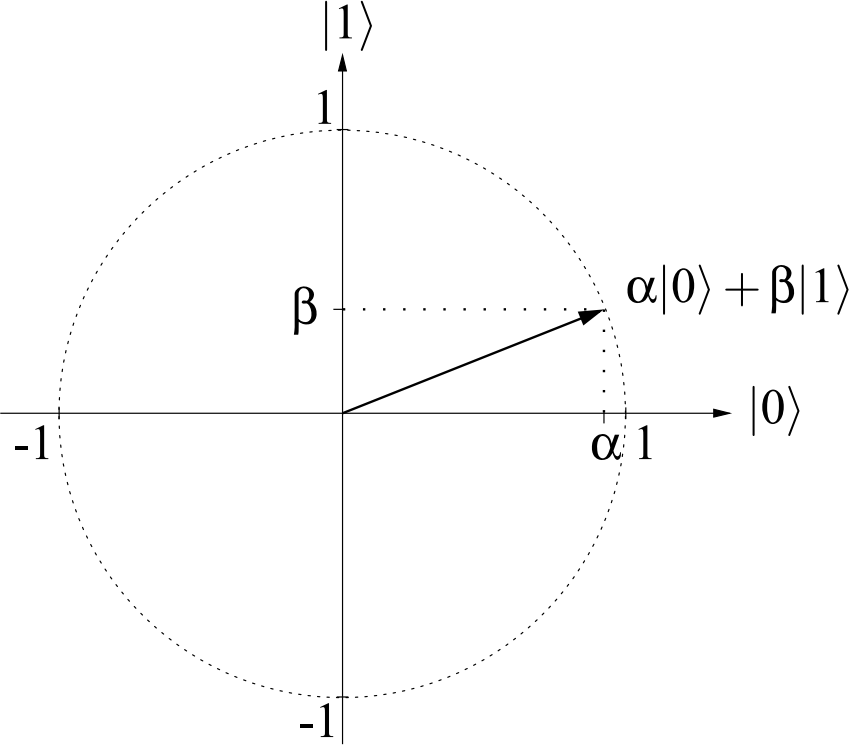
\includegraphics[width=0.5\linewidth]{img/Zustandsvektor_Standardbasis.png}
    \caption{Zustandsvektor in der Standardbasis}
    \label{fig:Standardbasis}
\end{figure}

Es wird ein Zustandsvektor in der Standardbasis dargestellt. Die Länge der Projektionen des Zustandsvektors auf den beiden Achsen bestimmen die Wahrscheinlichkeit, mit der, nach der Messung, einer der Zustände eingenommen wird. Mit der Wahrscheinlichkeit $\left|\alpha\right|^2$ wird der Zustand nach der Messung $\left|0\right.\rangle$ sein und mit der Wahrscheinlichkeit $\left|\beta\right|^2$ $\left|1\right.\rangle$. 

In der folgenden Abbildung wird derselbe Zustandsvektor gezeigt, mit dem Unterschied, dass die Koordinatenachsen nach der Hadamard-Basis ausgerichtet sind\footnote{\cite[S. 45]{homeister_quantum_2022}}.

\begin{figure}[h]
    \centering
    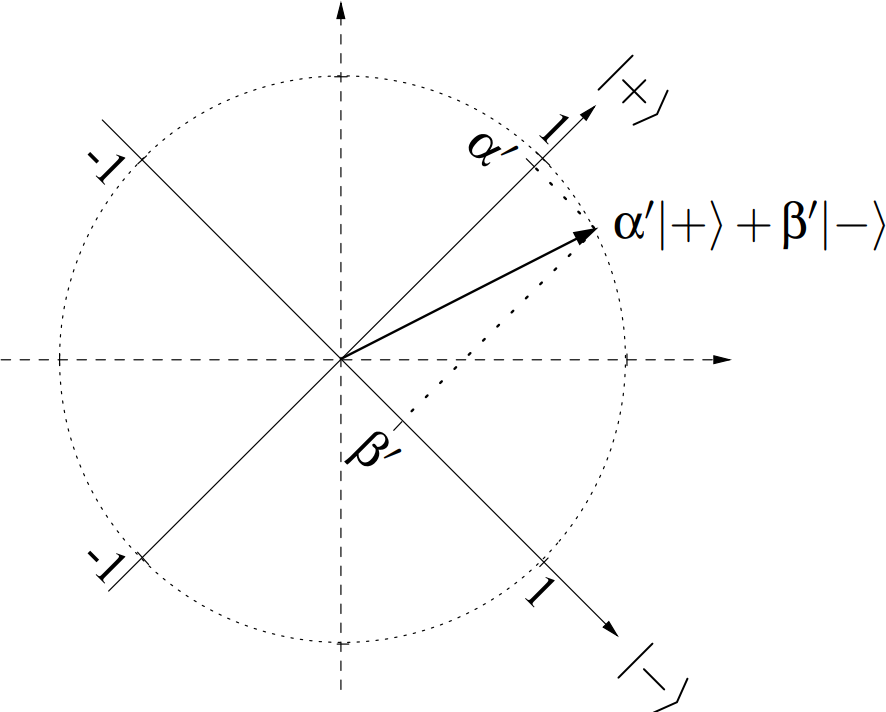
\includegraphics[width=0.5\linewidth]{img/Zustandsvektor_Hadamard-Basis.png}
    \caption{Zustandsvektor in der Hadamard-Basis}
    \label{fig:Hadamardbasis}
\end{figure}

Die Projektionen der Achsen haben sich im Vergleich zur Projektion auf die Standardbasis verändert. Mit der Wahrscheinlichkeit $\left|\alpha'\right|^2$ wird nach dem Messen der Zustand $\left|+\right.\rangle$ angenommen und mit der Wahrscheinlichkeit $\left|\beta'\right|^2$ $\left|-\right.\rangle$. 

Mathematisch sieht diese ``Basistransformation'' aus wie folgt:
\begin{equation}
    \alpha\left|0\right.\rangle+\beta\left|1\right.\rangle=\alpha'\frac{1}{\sqrt{2}}\left(\left|0\right.\rangle+\left|1\right.\rangle\right)+\beta'\frac{1}{\sqrt{2}}\left(\left|0\right.\rangle-\left|1\right.\rangle\right).
\end{equation}


Allgemeiner lässt sich zusammenfassen: ``Register R bestehe aus n Quantenbits und befinde sich im Zustand
$$\left|\phi\right.\rangle=\sum_{i=0}^{2^n-1}\alpha_i\left|i\right.\rangle$$
Wir messen bezüglich der Basis
$\left|0'\right.\rangle,\left|1'\right.\rangle,...,\left|(2^n-1)'\right.\rangle$
aus zueinander orthogonalen Vektoren der Länge 1.''\ \footnote{\cite[S. 46]{homeister_quantum_2022}} Dies ist eine andere Basis, als die in der sich $\left|\phi\right.\rangle$ befindet. ``Dabei wird die Superposition von $\left|\phi\right.\rangle$ zerstört. Hat $\left|\phi\right.\rangle$ bezüglich der Messbasis die Darstellung
$$\sum_{i=0}^{2^n-1}\alpha'_i\left|i\right.\rangle\verb|,|$$
so finden wir das Register nach der Messung mit Wahrscheinlichkeit $\left|\alpha'_i\right|^2$ im Zustand $\left|i'\right.\rangle$ vor.  Sämtliche anderen Informationen gehen dabei
verloren.''\ \footnote{\cite[S. 46]{homeister_quantum_2022}}\\

Das Messen einzelner Bits oder ganzer Register, sowie das Messen von Teilen eines Registers in der Standardbasis oder auch in einer anderen umfasst alles, was beim Messen möglich ist.


\section{Einführung in die Quanteninformatik 2}
\label{sec:einfuehrung-in-die-quanteninformatik-2}

\subsection{Drei Prinzipien des Quanten Computing}
\label{subsec:drei-prinzipien-des-quanten-computing}

Zusammenfassend lässt sich Quanten Computing auf drei wesentliche Prinzipien herunterbrechen.\\\\
Prinzip 1 - \textbf{Das Quantenregister}: Ein Quantenregister, das aus n-Qubits besteht, wird durch einen $2^n$-dimensionalen Vektorraum über komplexen Zahlen beschrieben.
Der Zustand eines solchen Registers ist eine Überlagerung (Superposition) aller möglichen Basiszustände.
Das bedeutet, dass das Register eine Kombination vieler möglicher Werte gleichzeitig annehmen kann.

Diese Fähigkeit der Superposition ist eine der Hauptstärken von Quantencomputern, da sie es ermöglichen, mehrere Berechnungen parallel durchzuführen.\\

Prinzip 2 - \textbf{Rechenschritte}: Rechenschritte in einem Quantencomputer basieren auf unitären Transformationen.
Diese Transformationen sind umkehrbar, was bedeutet, dass die Berechnung ohne Informationsverlust rückgängig gemacht werden kann.
Jede Operation kann lokal beschrieben werden, wobei nur zwei Qubits gleichzeitig beteiligt sind.

Diese Reversibilität der Rechenschritte stellt einen fundamentalen Unterschied zu klassischen Computern dar, bei denen Informationen während der Berechnung verloren gehen können.\\

Prinzip 3 - \textbf{Messungen}: Misst man den Zustand eines Quantenregisters, so erhält man als Ergebnis einen der Basiszustände mit einer Wahrscheinlichkeit, die aus der Amplitude dieses Zustands abgeleitet werden kann.

Die Messung verändert den Zustand des Systems auf den gemessenen Wert, sodass die ursprüngliche Superposition zerstört wird.\\

In diesen Prinzipien unterscheidet sich das Quanten Computing wesentlich von klassischen Computern.\\


\subsection{Verschränkung}
\label{subsec:verschraenkung}

Eine der interessantesten Eigenschaften von Quantenregistern ist die Verschränkung.
Bei der Verschränkung teilen sich zwei Qubits denselben Zustand.
Das heißt, messen wir den Zustand von Qubit 1, wissen wir auch sofort den Zustand von Qubit 2, ohne dieses gemessen zu haben.
Und was das Ganze noch faszinierender macht: Selbst über große Entfernungen zwischen den verschränkten Qubits bleibt die Eigenschaft der Verschränkung erhalten.
Dies bildet auch die Grundlage für die Quanten-Teleportation, auf die wir später noch zurückkommen.\\

\begin{tcolorbox}[title=Kommentar,
    title filled=false,
    colback=cyan!5!white,
    colframe=cyan!75!black]
    Die Verschränkung war mir bisher ein unbekanntes Konzept, welches sich nur sehr schwer greifen lässt.
    Dementsprechend schwierig war es auch, die Verschränkung zu verstehen und in eigenen Worten zu erklären.
    Besonders, dass diese unabhängig von der räumlichen Entfernung der Qubits erhalten bleibt.\\

    Dazu half mir ein kleines Beispiel: Stellen wir uns zwei Würfel vor, einen roten Würfel und einen blauen Würfel.
    Der blaue Würfel zeigt immer dieselbe Augenzahl wie der Rote.
    Wenn wir nun mit dem Roten würfeln und dieser eine 6 zeigt, wissen wir auch, dass der Blaue eine 6 zeigt, ohne diesen gewürfelt zu haben.
    Und das unabhängig davon, wie weit die beiden Würfel voneinander entfernt sind.
\end{tcolorbox}

Wie erzeugen wir eine solche Verschränkung?
Dazu betrachten wir exemplarisch ein Zwei-Bit-Register $\ket{b_{1}b_{2}}$ im Zustand $\ket{00}$.
Wir wenden auf das erste Bit die Hadamard-Transformation an und anschließend auf beide Bits die Operation CNOT\@.\\
\begin{equation}
    CNOT : \ket{x,y} \rightarrow \ket{x,y\oplus x}
\end{equation}\\

Das ergibt:\\
\begin{align}
    \ket{00} &\xrightarrow{H\otimes I_{2}} \frac{1}{\sqrt{2}}(\ket{0}+\ket{1})\ket{0} = \frac{1}{\sqrt{2}}(\ket{00}+\ket{10}) \\
    &\xrightarrow{CNOT} \frac{1}{\sqrt{2}}(\ket{00}+\ket{11})
\end{align}\\

Wenn wir nun das erste Bit messen, kommt mit einer Wahrscheinlichkeit 50\% das Ergebnis $\ket{0}$ mit dem Folgezustand $\ket{00}$ und mit einer Wahrscheinlichkeit von 50\% das Ergebnis $\ket{1}$ mit dem Folgezustand $\ket{11}$ heraus.
Wir wissen also nach der ersten Messung schon, bevor wir das zweite Qubit überhaupt gemessen haben, wie der Endzustand des Quantenregisters ist.
Und wie bereits zuvor erwähnt, bleibt diese Eigenschaft bei räumlicher Trennung der Qubits erhalten.
Hierbei ist auch zu erwähnen, dass es egal ist, welches der Qubits zuerst gemessen wird oder ob diese überhaupt gleichzeitig gemessen werden.\footnote{\cite[S. 76]{homeister_quantum_2022}}\\
\begin{figure}[H]
    \centering
    \includegraphics[width=0.8\textwidth]{img/Verschränkung Definition}
    \caption{Definition Verschränkung}
    \label{fig:verschraenkung}
\end{figure}

Diesen Zustand nennt man auch Bell-Zustand.
Es gibt insgesamt 4 solcher Bell-Zustände.
Diese beschreiben verschränkte Bits mit einer starken Kopplung (maximal verschränkt).\\
Daraus resultierend gibt es auch Verschränkungen mit einer weniger starken Kopplung.
Ein solcher Zustand könnte beispielsweise so aussehen:
\begin{equation}
    \ket{\phi} = 0.9\ket{00} + 0.1\ket{11}
\end{equation}\\

Hier sind die Qubits auch wieder miteinander verschränkt, allerdings sind die Wahrscheinlichkeiten für die Messergebnisse ungleich verteilt.
Das heißt, wir bekommen mit einer Wahrscheinlichkeit von 90\%, also sehr sicher, den Zustand $\ket{00}$ und nur mit 10\% den Zustand $\ket{11}$, also unsicher.
Diese weniger stark gekoppelten Qubits kommen in der Praxis häufiger vor, etwa durch äußere Einflüsse wie Rauschen oder Dekohärenz auf ehemals maximal verschränkte Qubits.
Das geht mit Leistungseinbußen einher, weshalb versucht wird, den Zustand der maximalen Verschränkung möglichst lange zu erhalten.\\


\subsection{Quantengatter \& Quantenschaltkreise}
\label{subsec:quantengatter-quantenschaltkreise}

„Klassische Schaltkreise bestehen aus Leitungen und Gattern.
Ganz analog bestehen Quantenschaltkreise aus Quantenleitungen und Quantengattern.
Jede Quantenleitung entspricht einem Quantenbit und ein Quantengatter führt eine unitäre Transformation aus.“\footnote{\cite[S. 76]{homeister_quantum_2022}}\\
\begin{figure}[H]
    \centering
    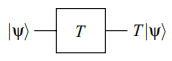
\includegraphics[width=0.35\textwidth]{img/Quantengatter Basic}
    \caption{Quantenschaltkreis}
    \label{fig:quantenschaltkreis}
\end{figure}

Wenn wir eine Berechnung mit mehreren Qubits ausführen, ergibt sich der Endzustand $\ket{x, y, z}$ aus dem Tensorprodukt der einzelnen Gatter\footnote{\cite[S. 76]{homeister_quantum_2022}}:
\begin{equation}
    (I_{2} \otimes W \otimes I_{2})(U \otimes V)\ket{x, y, z}
\end{equation}

\begin{figure}[H]
    \centering
    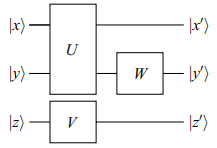
\includegraphics[width=0.35\textwidth]{img/Quantengatter 3er}
    \caption{Quantenschaltkreis mit Tensorprodukt}
    \label{fig:quantenschaltkreis-tensorprodukt}
\end{figure}

Da bei Quantenschaltkreisen die Umkehrbarkeit der Berechnungen garantiert werden muss, ist die Summe der Eingabe-Qubits gleich der Summe der Ausgabe-Qubits und pro Gatter dürfen höchsten 3 Qubits einbezogen werden.
Um dies zu gewährleisten, nutzen wir das Toffoli-Gatter, welches im nächsten Kapitel erläutert wird.
Außerdem können Qubits nicht kopiert werden, deshalb dürfen sich die Quantenleitungen nicht verzweigen und das Ergebnis eines Gatters nicht mehrfach verwendet werden.
Auf den Grund dafür kommen wir später nochmal zurück.\\

Eine der wichtigsten Operationen in der Quanteninformatik ist die Negation, genauer die kontrollierte Negation CNOT\@.
Dieses Gatter wird für alle Quantenoperationen benötigt, so zum Beispiel bei der Verschränkung.
Darstellen lässt es sich wie folgt:
\begin{equation}
    CNOT : \ket{x,y} \rightarrow \ket{x,y\oplus x}
\end{equation}

oder als Matrix:
\begin{equation}
    CNOT =
    \begin{pmatrix}
        1 & 0 & 0 & 0 \\
        0 & 1 & 0 & 0 \\
        0 & 0 & 0 & 1 \\
        0 & 0 & 1 & 0
    \end{pmatrix}
\end{equation}

Dieses CNOT-Gatter negiert nur dann das zweite Qubit, wenn das erste Qubit im Zustand $\ket{1}$ ist.\\

Weitere wichtige Operationen sind die Hadamard-Transformation, die wir bereits kennen, sowie die Pauli-Matrizen.
Die Pauli-Matrizen negieren ebenfalls, mithilfe einer unitären Transformation auf einem Bit.
Die bekannteste ist der „Bitflip“ X:\footnote{\cite[S. 79]{homeister_quantum_2022}}
\begin{equation}
    X =
    \begin{pmatrix}
        0 & 1 \\
        1 & 0
    \end{pmatrix}
\end{equation}

Die zwei weiteren Pauli-Matrizen sind der „Phasenflip“ Z:
\begin{equation}
    Z =
    \begin{pmatrix}
        1 & 0 \\
        0 & -1
    \end{pmatrix}
\end{equation}

und der „Y-Flip“ Y:
\begin{equation}
    Y =
    \begin{pmatrix}
        0 & -i \\
        i & 0
    \end{pmatrix}
\end{equation}

\begin{figure}[H]
    \centering
    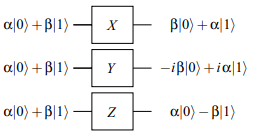
\includegraphics[width=0.5\textwidth]{img/Quantengatter Pauli_Matrizen}
    \caption{Pauli-Matrizen}
    \label{fig:pauli-matrizen}
\end{figure}

Durch die Kombination dieser drei Gatter CNOT, Hadamard-Transformation, sowie Pauli-Matrizen lassen sich alle Quantenberechnungen abbilden.
Sie bilden die grundlegendsten Rechenoperationen eines Quantencomputers.
Mit einem wesentlichen Unterschied zu logischen Gattern: Bei diesen lässt sich der Endzustand nicht unbedingt wieder in den Anfangszustand überführen.
Bei Quantengattern ist dies eine zwingende Voraussetzung, sie müssen umkehrbar sein.\\


\subsection{Umkehrbare Berechnungen}
\label{subsec:umkehrbare-berechnungen}

Wie bereits zuvor erwähnt, muss jede Rechenoperation eines Quantencomputers umkehrbar sein.
Es dürfen also keine Informationen gelöscht werden, wie es beispielsweise bei der Anwendung einer logischen AND-Operation passiert: aus zwei Eingabewerten wird ein Ausgabewert kombiniert.
So folgt aus 1 AND 0 = 0, jedoch ebenfalls aus 0 AND 0 = 0.
Sehen wir den Endzustand 0, wissen wir also nicht, welchen Zustand die beiden Bits zu Beginn hatten.
Das bedeutet, wir können Quantenrechenprozesse nicht auf dieselbe Art verarbeiten wie klassische Rechenprozesse.\\

Allerdings kann jede klassische Operation in eine umkehrbare Operation umgewandelt werden.
Veranschaulichen wir uns dies anhand des Toffoli-Gatters.\\

Das Toffoli-Gatter ist ein universelles, umkehrbares Gatter, welches AND, OR und NOT Operationen ersetzen kann.
Es besteht aus drei Eingabebits a, b, c und drei Ausgabebits a, b und $c\oplus(a\land b)$:\footnote{\cite[S. 87]{homeister_quantum_2022}}\\
\begin{figure}[H]
    \centering
    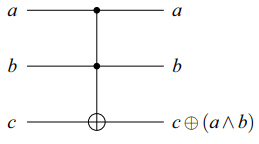
\includegraphics[width=0.35\textwidth]{img/Umkehrbare_Berechnungen Toffoli}
    \caption{Toffoli-Gatter}
    \label{fig:toffoli-gatter}
\end{figure}

Exemplarisch für AND: Wollen wir zum Beispiel ein Bit negieren, mit der Eingabe (a, b, c) = (1, 1, 0).
Dann ergibt die Rechnung über das Toffoli-Gatter (1, 1, 1), denn $(1\land 1) \oplus 0 = 1$.
Hier ist nun auch zu sehen, dass die Berechnung umkehrbar ist, wenn wir die Schritte einmal rückwärts gehen.
Dies ist genauso für die anderen Operatoren möglich, bedarf gegebenenfalls nur Umformung und den Einsatz mehrerer Toffoli-Gatter.\\

Auf diese Weise können wir jede klassische Rechenoperation umkehrbar gestalten, sodass diese auch für unsere Quantenschaltkreise nutzbar sind.\\


\subsection{Gestörte Berechnungen}
\label{subsec:gestoerte-berechnungen}

Wie wir bisher sehen konnten, scheint alles, was wir mit klassischen Computern berechnen, genauso effizient mit Quantencomputern berechenbar.
Warum also steht nicht bei jedem ein Quantenrechner zu Hause (wenn wir die Kosten mal außen vor lassen)?\\

Einer der Gründe dafür ist die Fehleranfälligkeit.
Während klassische Bits die Zustände 0 oder 1 abbilden, können Quantenbits bis zur Messung $\ket{0}$ oder $\ket{1}$ oder beide Zustände gleichzeitig annehmen.
Verdeutlichen wir, was das in der Praxis bedeutet: Nehmen wir an, der Zustand 0 eines klassischen Bits wird durch 0V und der Zustand 1 durch 5V dargestellt.
Nun kann es zu Spannungsschwankungen kommen und wir geben 4V statt 5V\@.
Da wir aber keinen Zustand für 4V haben, aber nur 2 Zustände abbilden können, können wir auch sagen, der Zustand 0 wir durch eine Spannung <2,5V abgebildet und der Zustand 1 durch >2,5V.
So liefert der Rechner uns auch weiterhin ein zuverlässiges Ergebnis, trotz Störung.\\

Die ist allerdings nicht für Quantenbits möglich, da wir nicht nur diese zwei Zustände abbilden.
Was bedeutet also hier eine Spannungsschwankung von 5V auf 4V?
Das wissen wir nicht, da bis zur Messung der Zustand nicht feststeht, so können wir also auch kein zuverlässiges Ergebnis mehr liefern.
So können selbst kleinste Störungen Quantenberechnungen verfälschen.
Zu beachten ist, dass bei einem gestörten Quantengitter sich der Fehler nur addiert.
Das heißt, der Fehler eines Gatters bleibt zwar in weiteren Berechnungen erhalten, jedoch wird er nicht größer.\\

Würden wir zum Beispiel ein Qubit durch 3 Quantengatter nacheinander umformen, wobei jedes dieser Gatter einen Fehler von 2\% hinzufügt, so beträgt der Fehler des Endzustands 6\%.
Das heißt, bei 50 Quantengattern welche einen Fehler von 2\% hinzufügen, beträgt der Fehler des Endzustands 100\%.
Wenn die Fehler nun aber exponentiell wachsen würden, hätten wir nach 3 Gattern einen Fehler von 8\%, nach 50 Gattern (theoretisch) einen Fehler von $2^{50}$\%.\\

Um die Frage vom Beginn des Kapitels nochmal aufzunehmen: Einer der Gründe, weshalb nicht jeder einen Quantencomputer zu Hause stehen hat, ist die Fehleranfälligkeit der Berechnungen.
Es bedarf großen Aufwands solche Fehler zu vermeiden und zu korrigieren.\\


\subsection{Grenzen}
\label{subsec:grenzen}

Angenommen in 10 Jahren ist das Problem der Dekohärenz gelöst, werden Quanten Computer die Lösung aller mathematischen Probleme sein?
Obwohl Quanten Computing noch mitten in der Entwicklung stecken, lässt sich jetzt schon absehen: Die Antwort darauf ist „Nein“.\\

\subsubsection{NP-vollständige Probleme}
\label{subsubsec:np-vollstaendige-probleme}
Eine der zentralen Fragen der Komplexitätstheorie beschäftigt sich mit NP-vollständigen Problemen.
Sie beschreibt Probleme, welche sich zwar leicht überprüfen lassen, doch algorithmisch mindestens eine exponentielle (O($2^{n}$), häufig sogar fakultative (O(n!)) Laufzeit haben.
Und würde man für ein NP-vollständiges Problem eine Lösung finden, also ein Algorithmus mit polynomieller O($n^{x}$) Laufzeit, so könnten alle dieser Probleme darauf umgeformt und gelöst werden.\\

Doch selbst Quantencomputer scheinen keine Lösung für diese Probleme finden zu können.
Das liegt daran, dass selbst Quantenalgorithmen, wie etwa der bekannte Shor-Algorithmus (zur Faktorisierung großer Zahlen),
oder der Grover-Algorithmus (zur unstrukturierten Suche in Datenbanken), zwar eine deutliche Geschwindigkeitsverbesserung im Vergleich zu klassischen Algorithmen bieten,
jedoch keine exponentielle Reduktion der Komplexität bei NP-vollständigen Problemen ermöglichen.\footnote{\cite[S. 165]{homeister_quantum_2022}}\\
Hier stoßen Quantencomputer also auf dieselben grundlegenden Herausforderungen wie klassische Computer.\\

\begin{tcolorbox}[title=Kommentar,
    title filled=false,
    colback=cyan!5!white,
    colframe=cyan!75!black]
    Wir hatten zunächst überlegt, den Grover- oder Shor-Algorithmus genauer zu beleuchten, haben uns dann aber dagegen entschieden,
    da wir uns auf die Grundlagen des Quanten Computing konzentrieren und uns nicht in einem komplexen Algorithmus verlieren wollten.\\

    Als wir mit dem Thema und der Recherche zur Quanteninformatik begonnen haben, war mir nicht bewusst, dass selbst Quantencomputer,
    welche noch in den Anfängen stecken und ein großes Potenzial bieten, schon jetzt an Grenzen stoßen, wie bei den NP-vollständigen Problemen.
    Es ist faszinierend zu sehen, dass selbst Quantencomputer, eine Technologie, die man sonst nur aus Sci-Fi Serien kennt, nicht alle mathematischen Probleme lösen kann.
\end{tcolorbox}

\subsubsection{Die perfekte Uhr}
\label{subsubsec:die-perfekte-uhr}
Ein weiteres Problem, auf welches Quantencomputer stoßen werden, ist die perfekte Zeitmessung, also die perfekte Uhr.
Jede Uhr hat zwei fundamentale Eigenschaften: Präzision und Zeitauflösung.
Die Zeitauflösung gibt an, wie klein die messbaren Zeitintervalle sind (also wie oft die Uhr tickt) und die Präzision gibt an, mit welcher Ungenauigkeit bei jedem Tick zu rechnen ist.
Ein Forscherteam hat gezeigt, dass es unmöglich ist gleichzeitig die perfekte Präzision und die perfekte Zeitauflösung zu erreichen.\\

Warum ist das wichtig für das Quanten Computing?
Aktuell haben Quantencomputer noch mit anderen Problemen, wie etwa der Dekohärenz oder Ungenauigkeiten bei den verwendeten Bauteilen zu kämpfen.
Allerdings zeigen Rechnungen, dass man nicht mehr so weit davon entfernt ist, bis die physikalische Grenze der Zeitrechnung die nächste Limitation für Geschwindigkeit und Zuverlässigkeit darstellt.\footnote{\cite{tuwien_grenzen_2023}}\\\\

\begin{tcolorbox}[title=Kommentar,
    title filled=false,
    colback=cyan!5!white,
    colframe=cyan!75!black]
    An der Stelle nur ein kleiner Ausblick auf die perfekte Uhr.
    Da ich bei meiner Recherche schnell in der Thermodynamik und Quantenmechanik gelandet bin und es ein umfangreiches physikalisches Wissen voraussetzt, vertiefe ich die perfekte Uhr nicht weiter.
\end{tcolorbox}


\subsection{Zukunft}
\label{subsec:zunft}

Wie sieht die Zukunft des Quanten Computing aus?
Was sind oder werden Anwendungsgebiete für diese Technologie sein?\\

\subsubsection{Quantum Machine Learning}
\label{subsubsec:quantum-machine-learning}
Künstliche Intelligenz oder auch Machine Learning sind zwei der Bereiche, in denen Quantencomputer eine große Rolle spielen könnten.
So schreibt die Fraunhofer-Allianz Big Data und Künstliche Intelligenz: \("\)Verfahren der künstlichen Intelligenz und des Machine Learnings lassen sich für Quantencomputer so anpassen, dass sie mehrere Lösungswege gleichzeitig beschreiten können.
Damit können Quantencomputer große Datenbestände in einem einzigen Schritt verarbeiten, Muster in den Daten aufspüren, die klassische Computer nicht entdecken und auch auf unvollständigen oder unsicheren Daten verlässliche Ergebnisse liefern.\("\)\footnote{\cite{tuwien_grenzen_2023}}
Quantencomputer könnten also die Lernverfahren von KI deutlich beschleunigen und verbessern.\\

Dies birgt allerdings auch ein Risiko, dessen ist sich auch das Bundesamt für Sicherheit in der Informationstechnik bewusst und gab in Kooperation mit Capgemini und dem Fraunhofer-Institut für Intelligente Analyse- und Informationssysteme eine Studie in Auftrag, die Quantum Machine Learning (QML) im Kontext von IT-Sicherheit untersuchen soll.\footnote{\cite{BSI_QUITS_2022}}
So hat QML beispielsweise großes Potenzial für die Malware und Spam Erkennung, sowie Kryptografie.
Gleichzeitig weiß man jetzt schon, dass aktuelle Verschlüsselungsmethoden, wie RSA oder ECC, durch Quantencomputer gebrochen werden können.
Daher wird bereits an quanten-resistenten Verschlüsselungsmethoden gearbeitet.\footnote{\cite{BSI_quantum_2022}}\\

\begin{tcolorbox}[title=Kommentar,
    title filled=false,
    colback=cyan!5!white,
    colframe=cyan!75!black]
    Die Studie des BSI ist tatsächlich sehr interessant zu lesen.
    Sie ist zwar von 2022, aber gibt einen guten Überblick über die Möglichkeiten und Risiken von Quantum Machine Learning.
\end{tcolorbox}

\subsubsection{Simulationen}
\label{subsubsec:simulationen}
Die Simulation von chemischen Molekülen.
Etwas bei dem selbst Supercomputer an ihre Grenzen stoßen.
Erstaunlicherweise ist die detaillierte Simulation von etwas so Kleinem wie Molekülen eine der größten Herausforderungen für unsere modernen Computer.
Hier könnten Quantencomputer Unterstützung leisten.
So schreibt das Fraunhofer Cluster of Excellence Cognitive Internet Technologies:
\("\) Mithilfe der Simulation von Molekülen könnten in Zukunft beispielsweise gezielt Katalysatoren entwickelt werden, die chemische Produktionsverfahren effizienter machen.
Chancen ähnlicher Größenordnung ergeben sich für die Pharmaindustrie.
Auch Forschung zu den im Angesicht des Klimawandels besondere relevanten Batterien zählt zum Anwendungsbereich der Simulation.\("\)\footnote{\cite{Fraunhofer_quantencomputing_2025}}
Deshalb erforscht das deutsche Zentrum für Luft- und Raumfahrt (DLR) zusammen mit dem Fraunhofer-Institut für Werkstoffmechanik IWM unter Verwendung des IBM-Quantencomputers neue Wege des Materialdesigns.\footnote{\cite{FraunhoferIWM_quantencomputer_2025}}\\

Neben den genannten Anwendungsgebiete wird außerdem ein Nutzer in der Logistik (optimaler Verteilung begrenzter Ressourcen), den Ingenieurswissenschaften und dem Finanzwesen (Risikoanalysen und Optimierung von Portfolios) gesehen.\footnote{\cite{Fraunhofer_quantencomputing_2025}}\\









\section{No Cloning Theorem} 
\label{sec:no-cloning}

Einer der faszinierendsten Aspekte der Quantenmechanik ist, dass es unmöglich ist
einen beliebigen unbekannten Quantenzustand perfekt zu duplizieren.
Dieses Konzept ist mit dem No-Cloning-Theorem beschrieben, einem grundlegenden Ergebnis der Quanteninformationstheorie.
Das Theorem hat nicht nur tiefgreifende Auswirkungen auf die Quanteninformatik und die Quantenkommunikation,
sondern auch für unser Verständnis der Natur der Information in Quantensystemen.\\

In der klassischen Physik ist die Vervielfältigung von Informationen einfach:
Ein Kopiergerät kann ein Dokument vervielfältigen, ohne das Original zu verändern.
In der Quantenmechanik wird dieser einfache Vorgang jedoch zu einer nicht trivialen und verbotenen Operation.
Das No-Cloning-Theorem besagt, dass es keine universelle Quantenoperation gibt
die eine identische Kopie eines beliebigen unbekannten Quantenzustands erzeugen kann.\\

In diesem Abschnitt werden wir das No-Cloning-Theorem aus verschiedenen Blickwinkeln betrachten, seinen Beweis diskutieren,
seine Konsequenzen untersuchen und verstehen, wie es die Landschaft der Quantentechnologien prägt.

\subsection{Definition}\label{subsec:definition}
Das No-Cloning-Theorem besagt, dass es unmöglich ist, eine identische Kopie eines unbekannten Quantenzustands zu erzeugen.
Mathematisch gesehen gibt es keinen unitären Operator $U$, der die folgende Bedingung erfüllt:
\begin{equation}
    U(\ket{\psi}\otimes\ket{e})=\ket{\psi}\otimes\ket{\psi}\label {eq:cloning_assertion}
\end{equation}
wobei $\ket{\psi}$ ein beliebiger Quantenzustand und $\ket{e}$ in Hilfszustand ist, der überschrieben werden soll.
Diese Gleichung drückt die Idee aus, dass, wenn wir den Operator $U$ auf den Zustand $\ket{\psi}$ anwenden
(kombiniert mit einem Hilfszustand), zwei Kopien des ursprünglichen Zustands entstehen sollten.
Das Theorem sagt uns, dass es für beliebige $\ket{\psi}$ keinen solchen Operator geben kann,
weil sich die Quanteninformation grundlegend von der klassischen Information unterscheidet.
\subsection{Beweis}\label{subsec:proof}
Als grundlegende Schlussfolgerung der Quantenmechanik gibt es mehrere Beweise für dieses Theorem.
Ein solcher Beweis, ein Widerspruchsbeweis, der der Einfachheit halber gewählt wurde, kann wie folgt definiert werden.

Zuerst nehmen wir zwei beliebige Quantenzustände, $\ket{\psi_1}$ und $\ket{\psi_2}$.
Dann werden diese beiden Zustände mit dem Klon operator $U$ geklont, den wir im vorigen Abschnitt definiert haben
und von dem wir für unseren Widerspruchsbeweis nun annehmen, dass er existiert.
\begin{equation}
\begin{split}
    U(\ket{\psi_1} \otimes \ket{e}) = \ket{\psi_1} \otimes \ket{\psi_1}\\
    U(\ket{\psi_2} \otimes \ket{e}) = \ket{\psi_2} \otimes \ket{\psi_2}
\end{split}\label{eq:clone_two_states}
\end{equation}

Mit dieser Information haben wir jetzt zwei Möglichkeiten, das Skalarprodukt von
$\braket{U(\psi_1 \otimes e)}{U(\psi_2 \otimes e)}$ zu schreiben.
Die eine verwendet das Ergebnis der vorherigen Gleichung, während die andere die Tatsache nutzt,
dass Quantenoperationen das Skalarprodukt ihrer Eingaben bewahren\footnote{\cite{segal_postulates_1947}}.

\begin{equation}
\begin{split}
    \braket{U(\psi_1 \otimes e)}{U(\psi_2 \otimes e)} = \braket{\psi_1 \otimes \psi_1}{\psi_2 \otimes \psi_2}\\
    \braket{U(\psi_1 \otimes e)}{U(\psi_2 \otimes e)} = \braket{\psi_1 \otimes e}{\psi_2 \otimes e}
\end{split}\label{eq:two_scalar_products}
\end{equation}

Einfache Ersetzung führt dann zur folgenden Gleichung
\begin{equation}
    \braket{\psi_1 \otimes \psi_1}{\psi_2 \otimes \psi_2} =
    \braket{\psi_1 \otimes e}{\psi_2 \otimes e}
\label{eq:tensor_equals}
\end{equation}

Da Tensor und Skalarprodukte kompatible sind\footnote{\cite{segal_postulates_1947}} simplifiziert das weiter zu:

\begin{equation}
    \braket{\psi_1}{\psi_2}\braket{\psi_1}{\psi_2}=\braket{\psi_1}{\psi_2}\braket{e}{e}
    \label{eq:scalar_equals}
\end{equation}

Und schließlich, weil für jeden Zustand $\ket{e}$ die Gleichung $\braket{e}{e} = 1$ gilt, kommen wir zu dieser Gleichung:

\begin{equation}
    \braket{\psi_1}{\psi_2}^2 = \braket{\psi_1}{\psi_2}
    \label{eq:square_equals_single}
\end{equation}

Es sollte nun offensichtlich sein, dass diese Gleichung nur zwei Lösungen hat:
$\braket{\psi_1}{\psi_2} = 1$ or $\braket{\psi_1}{\psi_2} = 0$.
Die erste Lösung impliziert, dass $\psi_1 = \psi_2$, was für eine allgemeine Klon-Operation nicht hilfreich ist, erlaubt aber eine
Operation, die Kopien eines bestimmten Zustands erzeugt.
Das ist vor allem nützlich um Quantensysteme in einen bekannten Zustand zu initialisieren.
Die zweite Lösung erlaubt zwar, dass sich $\psi_1$ und $\psi_2$ unterscheiden, und ist damit auf den ersten Blick
vielversprechend, verlangt aber immer noch, dass die beiden Zustände orthogonal zueinander sind.
Das ist zwar weniger restriktiv als die erste Lösung, erlaubt aber immer noch nur eine Operation, die eine bestimmte Klasse
von Zuständen kopieren kann, von der alle Mitglieder zueinander orthogonal sind.
Somit ist auch mit dieser Lösung keine allgemeine Klon-Operation möglich.
\subsection{Folgen}\label{subsec:implications}
Das No-Cloning-Theorem hat weitreichende Auswirkungen auf eine Reihe von Gebieten der
Quantenmechanik und Quanteninformatik.

\subsubsection{Quantenkommunikation}
In der klassischen Informationstheorie ist das Kopieren von Daten eine zentrale Technik, um Information zu vervielfältigen und zu übertragen.
Bei klassischen Bits kann man exakt den gleichen Wert duplizieren, indem man eine Kopie eines Bits erstellt.
Im Gegensatz dazu verhindert das No-Cloning-Theorem das Erstellen von exakten Kopien von Quantenbits (Qubits).\\

Das bedeutet, dass im Bereich der Quantenkommunikation, insbesondere bei der Quantenkryptographie, ein Angreifer,
der versucht die Quanteninformation abzufangen oder zu kopieren, in der Regel Fehler einführen wird, die entdeckt werden können.
Dieses Prinzip bildet die Grundlage für Sicherheitsprotokolle wie Quantum Key Distribution (QKD),
bei denen ein Abhörversuch die Übertragung zerstören würde und somit leicht zu erkennen ist.

\subsubsection{Schutz der Quanteninformation}
Da das No-Cloning-Theorem das exakte Kopieren eines unbekannten Zustands verbietet,
wird auch die Quanteninformation von Natur aus gegen bestimmte Arten von Angriffen geschützt.
In klassischen Computersystemen kann ein Angreifer beliebig viele Kopien von Information erstellen,
um sie zu analysieren und gegebenenfalls zu entschlüsseln.
In einem quantenmechanischen System jedoch kann ein Datenexfiltrationsversuch oder das Kopieren eines Zustands
nicht ohne weiteres erfolgen, ohne dass der Versuch des Kopierens den Zustand verändert
und die Quanteninformation damit entwertet wird.\\

Ein gutes Beispiel für diese Art von Sicherheit ist das BB84-Protokoll für Quantenkryptographie.
Bei der Quantenverschlüsselung wird eine Nachricht durch verschränkte Quantenbits übertragen.
Jeder Versuch, die Nachricht zu kopieren oder abzufangen, verändert den Zustand der Qubits und wird vom Empfänger erkannt.

\subsubsection{Design von Algorithmen}

Das No-Cloning-Theorem hat auch tiefgehende Auswirkungen auf das Quantencomputing.
In klassischen Computern ist das Kopieren von Informationen eine grundlegende Technik, die in vielen Algorithmen und Protokollen verwendet wird.
Quantencomputer hingegen können keine exakten Kopien eines Zustands herstellen, was bedeutet,
dass traditionelle Techniken wie fehlerkorrigierende Codes, die in klassischen Computern üblich sind, in der Quantenwelt nicht direkt anwendbar sind.\\

Allerdings existieren spezielle Quantenfehlerkorrekturcodes, die darauf ausgelegt sind, Fehler zu korrigieren,
die durch das Fehlen einer exakten Kopierbarkeit von Quanteninformation entstehen.
Diese Codes erfordern jedoch eine zusätzliche Anzahl von Qubits und eine komplexe Fehlerkorrekturstrategie,
was das Quantencomputing technisch anspruchsvoll macht.
Trotzdem sind Quantenfehlerkorrekturmethoden von entscheidender Bedeutung für die zukünftige Skalierbarkeit
und Zuverlässigkeit von Quantencomputern und werden später in diesem Artikel genauer beschrieben[\ref{sub:quantum_error_correction}].

\begin{tcolorbox}[title=Kommentar,
    title filled=false,
    colback=cyan!5!white,
    colframe=cyan!75!black]
Verschiedene Messmethoden
Jeder Quantenalgorithmus ist auch grundsätzlich anders als ein klassischer Algorithmus, da Operationen anders implementiert
werden müssen, auch wenn die Theorie des Algorithmus identisch zu einem klassischen Algorithmus ist.
    Dieser Aspekt wird hier allerdings nicht näher behandelt werden.
\end{tcolorbox}

\subsubsection{Speicherung von Quanteninformation}
Das No-Cloning-Theorem hat weitreichende Konsequenzen für die Quanteninformationstheorie,
insbesondere für die Konzepte der Informationsspeicherung und -übertragung.
Die Unmöglichkeit des Klonens ist eng mit den grundlegenden Prinzipien der Quantenmechanik wie Überlagerung und Verschränkung verknüpft.
Sie hindert die Schaffung von perfekten Kopien von Quanteninformation und erfordert, dass Information auf neue, kreative Weise verarbeitet und gespeichert wird.\\

Ein interessantes Beispiel sind die Quantenlogikgatter, die in Quantencomputern verwendet werden.
Diese Gatter müssen mit den Einschränkungen des No-Cloning-Theorems arbeiten und können keine klassischen,
deterministischen Kopien erzeugen, sondern müssen die Quanteninformation in verschränkten oder überlagerten Zuständen manipulieren.

\subsubsection{Messungen und Messgenauigkeit}

In der Quantenmetrologie, die sich mit der präzisen Messung von quantenmechanischen Systemen beschäftigt,
beeinflusst das No-Cloning-Theorem ebenfalls die Art und Weise, wie Messungen durchgeführt werden können.
Da das exakte Kopieren von Zuständen nicht möglich ist, kann das Präzisionsmaß für Messungen nicht durch das
Vervielfachen von Messinstrumenten oder durch das Erstellen von Kopien von Quantenobjekten verbessert werden.
Stattdessen wird die Quantenmessung durch andere Techniken wie
Quanteninterferometrie und den Einsatz von verschränkten Zuständen optimiert.




\section{Quantenteleportation}\label{sec:quantum-teleportation}

\subsection{Einführung}\label{subsec:introduction}
Quantenteleportation ist ein bahnbrechendes Phänomen, das die Übertragung von Quanteninformationen
zwischen zwei entfernten Orten ermöglicht, ohne dass das Teilchen oder Objekt, das die Information trägt, physisch bewegt wird.
Im Gegensatz zur theoretischen klassischen Teleportation, bei der es um den Transport von Materie oder Energie geht,
konzentriert sich die Quantenteleportation auf die Übertragung von Quantenzuständen.
Dieser Prozess nutzt die Prinzipien der Quantenmechanik, einschließlich Verschränkung, Superposition,
und das No-Cloning-Theorem,
um den Zustand eines Quantenobjekts (z.B.\ eines Photons oder eines Elektrons) von einem Ort zum anderen zu übertragen.
Dabei spielt die Entfernung der Objekte keine Rolle.\\

Der Begriff ``Quantenteleportation'' kann etwas irreführend sein, da bei diesem Prozess keine eigentliche Materie teleportiert wird.
Was stattdessen ``teleportiert'' wird, ist die Information über den Quantenzustand eines Teilchens.
Der Schlüssel zur Quantenteleportation ist die Quantenverschränkung,
ein Phänomen, bei dem zwei oder mehr Teilchen so miteinander korrelieren, dass der Zustand des einen Teilchens den Zustand des anderen augenblicklich
 beeinflusst, unabhängig davon, wie weit sie voneinander entfernt sind.
Diese ``gespenstische Fernwirkung'', wie Albert Einstein sie nannte,
ermöglicht die Übertragung von Quanteninformation zwischen weit entfernten Parteien, ohne dass die oft fragilen Quantenzustände selbst transportiert werden müssen.

\subsection{Aufbau}\label{subsec:setup}

Es muss ein Quanten-Verschränkungspaar vorhanden sein.
Dieses Paar muss sich im Bell-Zustand\cite{quantuminfocambridge} befinden, um sicherzustellen, dass die Messung des einen den Zustand des anderen beeinflusst.
Dieses Paar wird in der Regel durch einen Prozess wie
Spontane parametrische Abwärtsumwandlung\cite{couteau2018spontaneous} erzeugt.
Derzeit werden dafür in der Regel einfache Photonen oder Ionen verwendet.\\


Außerdem müssen sich an den Endpunkten der Teleportation zwei Parteien befinden, im Folgenden Alice und Bob genannt, die beide in der Lage sind, mit Quantensystemen zu interagieren und Messungen vorzunehmen, was normalerweise einen Quantencomputer mit begrenzter Funktionalität bedeutet.
Schließlich muss ein klassischer Kommunikationskanal zwischen Alice und Bob bestehen.
Der Schlüssel für die Quantenteleportation ist hier, dass dieser Kanal nicht in der Lage sein muss, Quantenzustände zu transportieren - dafür ist die Teleportation gedacht -, sondern nur herkömmliche Bits.

%<Diagramm Aufbau>

\subsection{Vorgang}\label{subsec:process}

Nachdem der Aufbau abgeschlossen ist, stellt sich nun die Frage, was tatsächlich getan werden muss, um die Quantenteleportation durchzuführen.
Dies kann in mehrere Schritte aufgeteilt werden.

\subsubsection{Alices Bell Zustand Messung}
Der erste Schritt, den Alice durchführt, ist die Bell-State-Messung, die zwei wichtige Teilschritte umfasst.

Zunächst kombiniert Alice das Teilchen, das sie teleportieren möchte, mit ihrer Hälfte des verschränkten Paares.
Dies geschieht in der Regel mithilfe eines Strahlenteilers oder eines Interferometers, um die beiden Teilchen in einen Superpositionszustand zu versetzen.

Zweitens misst Alice die beiden kombinierten Teilchen in der Bell-Basis, die die Teilchen aus ihren vier möglichen Zuständen in einen einzigen zusammenfallen lässt.
Diese Messung ist entscheidend, denn sie bestimmt, wie Bob sein Teilchen anpassen muss, um den Zustand wiederherzustellen, den
Alice teleportiert.
\subsubsection{Klassische Kommunikation}
Als Nächstes verwendet Alice ihren klassischen Kommunikationskanal, um ihre Messung an Bob zu senden.
Dies erfordert die Übertragung von nur zwei Bits (den beobachteten Zustand des zu teleportierenden Qubits und den beobachteten Zustand des
des verschränkten Paares), was für keinen Kommunikationskanal ein Problem darstellen sollte.
Diese geringe Bandbreitenanforderung in der klassischen Kommunikation macht in der Tat mehrere Kommunikationskanäle verfügbar
die normalerweise wegen ihrer geringen Bandbreite nicht infrage kämen, insbesondere wenn die Teleportation über große
Entfernungen stattfinden soll.
Diese Information reicht jedoch aus, um Bob zu instruieren, wie er sein eigenes System einstellen muss.
\subsubsection{Bobs Quantenoperation}
Nun, da Bob die klassische Messung erhalten hat, muss er eine oder beide (je nach Messung) der folgenden Methoden anwenden: Das
Pauli-X-Gatter für einen Bit-Flip oder das Pauli-Z-Gatter für einen Phasen-Flip.
Durch diese Operation wird sein Quantenzustand in denselben Zustand versetzt, den Alices Quantenteilchen hatten, bevor ihre
Messung die Superposition kollabierte.
Hier ist auch noch einmal darauf hinzuweisen, dass Bob den Zustand erst erstellt, nachdem Alice ihn mit der Messung
bereits zerstört hat - wie das No-Cloning-Theorem besagt\ref{sec:no-cloning} wird der Zustand nie kopiert, sondern nur
übertragen.

Sobald Bob dies getan hat, ist die Quantenteleportation abgeschlossen.
\subsection{Mathematik}\label{subsec:proof2}

\subsubsection{Verschränkung und Bell-Zustände}

Zu Beginn des Prozesses haben wir zwei Teilchen (Teilchen 2 und 3), die sich an den Orten A und B befinden.
Diese Teilchen werden in einem verschränkten Zustand (Bell-Zustand) erzeugt.
Ein Bell-Zustand ist eine der vier möglichen maximal verschränkten Zustände, die ein Paar von Quantenobjekten haben kann.
Ein Beispiel für einen solchen Zustand ist:

\begin{equation}
|\Phi^+\rangle = \frac{1}{\sqrt{2}} \left( |00\rangle + |11\rangle \right)
\end{equation}

Dieser Zustand wird zwischen den beiden Teilchen 2 und 3 geteilt, wobei Teilchen 2 bei A und Teilchen 3 bei B ist.

\subsubsection{Der zu teleportierende Zustand}

Nun nehmen wir an, dass wir den Zustand eines dritten Teilchens (Teilchen 1) teleportieren möchten, das sich am Ort A befindet. Der Zustand des Teilchens 1 kann allgemein als:

\[
|\psi\rangle_1 = \alpha |0\rangle + \beta |1\rangle
\]

ausgedrückt werden, wobei \(\alpha\) und \(\beta\) komplexe Zahlen sind, die den Zustand beschreiben.

\subsubsection{Verschränkung und Messung}

Der gesamte Zustand des Systems (Teilchen 1, 2 und 3) kann als Produktzustand von Teilchen 1 und dem verschränkten Zustand von Teilchen 2 und 3 beschrieben werden:

\[
|\Psi\rangle_{123} = |\psi\rangle_1 \otimes |\Phi^+\rangle_{23} = \frac{1}{\sqrt{2}} \left( \alpha |0\rangle_1 + \beta |1\rangle_1 \right) \otimes \left( |00\rangle_{23} + |11\rangle_{23} \right)
\]

Durch Anwenden der Distributivität ergibt sich:

\begin{gather*}
    |\Psi\rangle_{123} = \frac{1}{\sqrt{2}} \left( \alpha |0\rangle_1 \otimes (|00\rangle_{23} + |11\rangle_{23}) + \beta |1\rangle_1 \otimes (|00\rangle_{23} + |11\rangle_{23}) \right)\\
    |\Psi\rangle_{123} = \frac{1}{\sqrt{2}} \left( \alpha |000\rangle_{123} + \alpha |011\rangle_{123} + \beta |100\rangle_{123} + \beta |111\rangle_{123} \right)\\
\end{gather*}

Nun wird eine Bell-Zustandsmessung auf den Teilchen 1 und 2 durchgeführt, die den Zustand des Systems in einen der vier Bell-Zustände projiziert. Die Messung ist zufällig, und die Ergebnisse können durch die folgenden Zustände beschrieben werden:

\[
|\Phi^+\rangle_{12}, |\Phi^-\rangle_{12}, |\Psi^+\rangle_{12}, |\Psi^-\rangle_{12}
\]

\subsubsection*{Klassische Kommunikation und Zustandserstellung}

Nachdem die Messung durchgeführt wurde, sendet der Ort A das Messresultat an Ort B über einen klassischen Kanal.
Anhand der Nachricht kann Ort B den Zustand des Teilchens 3 (das ursprünglich am Ort B war) in den gewünschten Zustand \(|\psi\rangle_1\) transformieren. Dazu wird eine der folgenden Operationen durchgeführt, abhängig von der Messung, die an Ort A durchgeführt wurde:

\begin{gather*}
    |0\rangle_3 \quad \text{(falls Messung das Ergebnis } |\Phi^+\rangle\text{ ergibt)}\\
    X|0\rangle_3 \quad \text{(falls Messung das Ergebnis } |\Phi^-\rangle\text{ ergibt)}\\
    Z|0\rangle_3 \quad \text{(falls Messung das Ergebnis } |\Psi^+\rangle\text{ ergibt)}\\
    XZ|0\rangle_3 \quad \text{(falls Messung das Ergebnis } |\Psi^-\rangle\text{ ergibt)}\\
\end{gather*}

Durch diese Operationen wird der Zustand des Teilchens 3 in den ursprünglichen Zustand von Teilchen 1 (\( \alpha |0\rangle + \beta |1\rangle \)) überführt.


\subsection{Herausforderungen}\label{subsec:challenges}
Obwohl die Quantenteleportation ein vielversprechender Forschungszweig ist, gibt es noch einige Herausforderungen zu bewältigen

\subsubsection{Verschränkung Erzeugen und Erhalten}
Eine der größten Herausforderung ist die Erzeugung und Erhaltung eines verschränkten Systems zwischen dem Start- und Zielpunkt
der Teleportation.
Die Teleportation ist zwar theoretisch nicht durch Entfernung begrenzt, aber je größer die Entfernung zwischen den Orten
des do schwieriger ist es die verschränkten Teilchen aufzuteilen, ohne die Verschränkung zu beschädigen.\\

Ein Lösungsansatz sind hier Quantenrepeater: Spezialisierte Geräte die die Entfernung zwischen direkt verschränkten Teilchen reduzieren,
indem sie diese nur zwischen Repeater Stationen aufteilen müssen.
In der Station werden dann mithilfe von Entanglement Swapping zwei Verbindungen des Repeaters verschränkt.

\subsubsection{Klassische Kommunikation}
Auch wenn die benötigte Bandbreite der klassischen Kommunikation minimal ist, muss trotzdem ein Kommunikationskanal
existieren.
Das hat zwei signifikante Nachteile: Zum einen ist die klassische Kommunikation auf die Lichtgeschwindigkeit begrenzt,
was ein Geschwindigkeitslimit für die Teleportation erzeugt, auch wenn die ``spukhafte Fernwirkung'' der Quantenmechanik
schneller passieren könnte\cite{hensen2015loophole}.
Zum anderen sind klassische Kommunikationskanäle anfällig für Observation - ein Angreifer kann zwar
ohne das verschränkte Teilchen den Quantenzustand nicht reproduzieren ist aber in der Lage festzustellen, dass die
Kommunikation stattgefunden hat.
Ebenfalls könnte der Angreifer auch die Kommunikation stören, was zwar bei geeigneten Protokollen den Teilnehmern
offensichtlich ist aber trotzdem eine Schwachstelle darstellt.
Die einzige bekannte Lösung ist hier ein robustes klassisches Kommunikationssystem, was für andere Kommunikationszwecke
bereits aufgebaut ist oder wird, aber leider die Lichtgeschwindigkeitslimitation nicht umgehen kann.


\subsubsection{Skalierbarkeit}

Ein weiteres bedeutendes Problem der Quantenteleportation ist die Skalierbarkeit.
Während die Quantenteleportation in kleinen, kontrollierten Systemen von einigen wenigen Qubits relativ einfach durchgeführt werden kann,
stellt die Skalierung auf größere Netzwerke und damit nützliche Datenmengen und die Integration in reale Kommunikationssysteme eine enorme Herausforderung dar.
Um Quantenteleportation praktisch nutzen zu können würde es ein großflächiges System von Kommunikationskomponenten
benötigen.
Die Erstellung dieser bräuchte Quantentechnologien in einer Menge in der diese momentan weder technisch möglich
noch finanziell tragbar ist, wenn man bestehende Preise hochrechnet.\\

Hier ist allerdings die Erwartung, dass weitere Forschung dieses Problem beheben wird.
Es wird sowohl an günstigeren Methoden zur Erstellung von verschränkten Systemen und der Stabilisierung dieser,
als auch an der Erstellung von Quantenkomponenten rege geforscht.
Auch an Forschungsbudget fehlt es hier nicht, da einige große Technologiefirmen wie Google und Microsoft an Quantentechnologie forschen.

\subsubsection{Fehlerquellen und Messgenauigkeit}
Die Messgenauigkeit ist entscheidend für die erfolgreiche Durchführung der Quantenteleportation.
Eine fehlerhafte Messung der Bell-Zustände kann dazu führen, dass der teleportierte Zustand nicht korrekt wiederhergestellt werden kann.
Fehlerquellen können in den Messinstrumenten, in der Kommunikation oder auch in der Quantenverschränkung selbst liegen.

Auch hier wird rege geforscht, da alle drei Aspekte nicht eigen zur Quantenteleportation sind, sondern nahezu alle
Quantenoperationen betreffen.



  
\section{Quantenhardware}
\label{sec:quantenhardware}

Die Realisierung eines Quantencomputers ist durch hohe technische herausforderungen geprägt. Um die besonderen Eigenschaften der Qubits eines Quantencomputers, wie Superposition und Verschränkung, nutzen zu können, müssen sie durch externe Einflüsse geschützt werden und die Dekoheränz minimiert werden.
Äußere Einflüsse wie Temperaturschwankungen, elektromagnetische Felder oder Strahlung aller Art können die Qubits beeinflussen. Aus diesem Grund werden Quantencomputer bei extrem niedrigen Temperaturen und in einem Vakuum betrieben.\\

Außerdem ist nicht nur die Herstellung der Qubits eine Herausforderung, sondern auch die Steuerung, Auslesung und Korrektheit von physikalischen Qubits.

\subsection{Dekohärenz}
\label{sub:dekohaerenz}
Dekoheränz ist ein zentrales Konzept, welches wichtig in der Entwicklung von Quantencomputern ist. Der Prozess der Dekoheränz beschreibt den Verlust der koheränten Quanteneigentschaften eines Qubits durch Wechselwirkung mit der Umgebung.
Diese Veränderung führt zu einem Übergang von quantenmechanischem Verhalten zu einem klassischem Verhalten von Bits.\\

In der Quantenmechanik können Systeme in Überlagerungszuständen existieren, wobei mehrere Zustände gleichzeitig eingenommen werden können. Diese Eigenschaft erklärt auch das Phänomen der Quanteninterferenz.
Äußere Einflüsse durch die Umgebung kann eine Verschränkung von Qubits zerstören. Dies führt dazu, dass die Phasenbeziehungen zwischen den Qubits beeinflusst oder gar aufgehoben werden.
Folgernd verliert das System die Interferenzeffekte und verhält sich zunehmend klassischer. Diese Zeit nennt man Dekoheränzzeit.\\

Die \textbf{Dekoheränzzeit} ($T_2$) eines Qubits misst die Länge der Zeit, in der er in der Lage bleibt kohärent zu bleiben, welcher danach von äußeren Einflüssen zerstört wird.
Neben $T_2$ wird auch häufig die \textbf{Relaxationszeit} ($T_1$) gemessen, welche angibt, wie lange ein Qbit im angeregten Zustand bleibt, bevor es auf sein Grundzustand zurückfällt.
In der Realität ist die Dekoheränzzeit jedoch in den meisten Fällen kürzer als die Relaxationszeit.\\

\textbf{Berechnung der Dekoheränzzeit}\\
Durch eine Messung der zeitlichen Abnahme der Koheränz eines beispielhaften Qubits kann die Dekoheränzzeit eines Systems festgelegt werden.
Bei einem Quantencomputer, der auf dem Spin eines Teilchen beruht, kann dies durch die \textbf{Spin-Echo-Methode} gemessen werden.
Quantencomputer, die auf anderen Qubits basieren, haben equivalente Methoden um die Kohärenz zu messen.\\

Das einfachste Modell zur Beschreibung der Dekoheränzzeit ist die \textbf{Exponentielle Abnahme der Kohärenz}

\begin{equation}
    C(t) = C(0)*e^{-t/T_2}
\end{equation}

Dabei ist:\\
$C(t)$ Die Kohärenz des Qubits zum Zeitpunkt t\\
$C(0)$ Die initiale Koheränz\\
$T_2$ Die Dekoheränzzeit\\

Indem man den Kohärenzverlust experimentell misst und die Werte in eine exponentielle Abklingfunktion einpasst, erhält man $T_2$\\

\begin{tcolorbox}[title=Kommentar,
    title filled=false,
    colback=cyan!5!white,
    colframe=cyan!75!black]
    Die \textbf{Dekoheränzzeit} kann auch durch genauere jedoch auch deutlich kompliziertere weise errechnet werden.
    Bekannte Methoden hierfür wären zum Beispiel die Spektrale Analyse, Dynamische Entkopplung, Hahn-Echo und Ramsey-Interferometrie.
    Außerdem wird duch das häufige messen der Dekoheränzzeit diese indirekt verlänger. Diesen Effekt nennt man Quanten-Zeno-Effekt.\\
    Zuletzt muss auch die Lindblad-Gleichung genannt werden welche den Zeitverlauf der Dichtematrix in einem Offenen Quantensystem beschreibt.
    \begin{equation}
        \frac{dp}{dt} = -i[H,p]+\sum_i(L_ipL^\dagger_i-\frac{1}{2}\{L^\dagger_i L_i,p\})
    \end{equation}
    Diese Themen sprengen jedoch den Rahmen dieser Arbeit in Richtung Physik und werden deswegen nicht weiter behandelt.
\end{tcolorbox}

\subsection{Universelle Quantencomputer}
\label{sub:universelle_quantencomputer}
Universelle Quantencomputer beruhen grundlegend auf einem Gatter Modell, wie bereits in diesem Artikel beschrieben. Folgend sind drei der meist erforschten
Methoden, welche dieses Modell physikalisch umsetzen.\\

Ein prominentes Beispiel für die Umsetzung eines universellen Quantencomputers ist der \textbf{Sycamore Chip}, welcher auf supraleitenden Qubits basiert.
Dieser Chip ist in einem Gatter angeordnet für die Kommunikation zwischen Qubits und die durchführung von Quantenoperationen.\\

\begin{figure}[H]
    \centering
    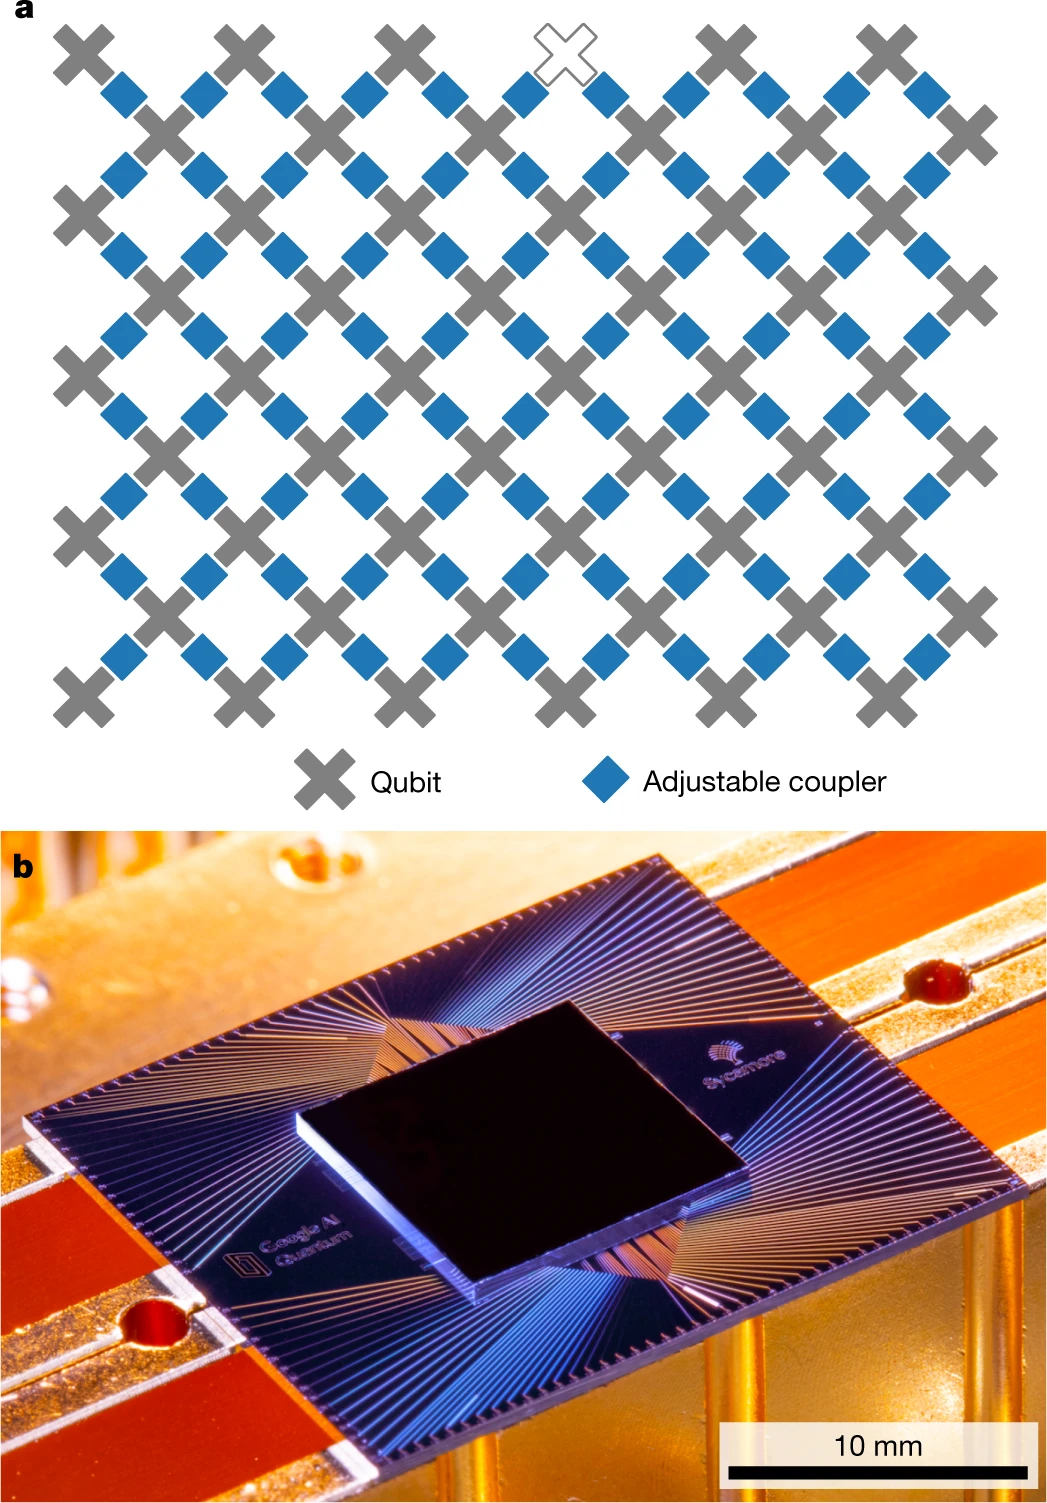
\includegraphics[width=0.7\linewidth]{img/SycamoreChip.png}
    \caption{Sycamore Chip von Google}
    \label{fig:Sycamore}
\end{figure}

\subsubsection{Supraleitende Qubits}
\label{subsub:superleiter}
Quantencomputer mit Supraleitern funktionieren mit elektrischen Schaltkreisen, die bei Temperaturen nahe dem absoluten Nullpunkt betrieben werden. Solche Temperaturen sind nötig,
um die supraleitende Eigenschaft aufrecht zu erhalten.\\

Zwei häufig benutze Qubit-Typen dieser elektrischen Schaltkreise sind:\\
\textbf{Transmon-Qubits}, basiert auf der Ladung des Energieniveaus, welche durch eine Josephson-Junktion kontrolliert wird.\\
\textbf{Flux-Qubits} werden auch durch Josephson-Junktions kontrolliert, beruhen jedoch auf dem magnetischen Fluss in der Schleife.\\

Beide Ansätze basieren auf dem \textbf{Josephson-Effekt}, welcher auftritt, wenn ein supraleitender Strom durch eine dünne Isolierschicht zwischen zwei Supraleitern fließt.\\
Dieser Effekt hat zur Folge, dass eine nichtlineare Spannung-Stom-Beziehung entsteht und für die Manipulation von Qubits genutzt wird.\\

\begin{figure}[H]
    \centering
    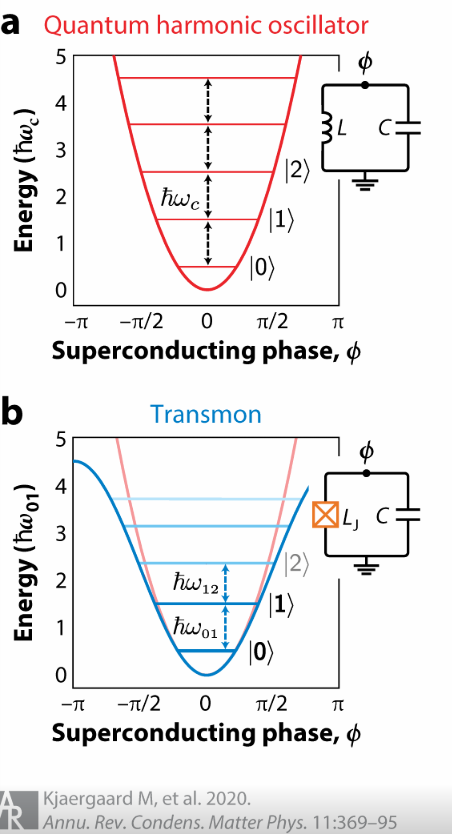
\includegraphics[width=0.75\linewidth]{img/JJ.png}
    \caption{Josephson-Effekt mit einem Josephson Junktion}
    \label{fig:Josephson-junktion}
\end{figure}

In der vorliegenden Abbildung wird der Unterschied zwischen einer harmonischen Quantenschwankung (a) und der nichtlinearen Schwankung des Energie Niveaus der Josephson Junktion (b) abgebildet.\\

Der Phasenunterschied bei der harmonischen Oscellation, gekennzeichnet als $\hbar\omega_c$, ist identisch. Auf der Abbildung ist zu sehen, dass das Energieniveau der Phasen zwischen $\ket{0} \leftrightarrow \ket{1}$
und $\ket{1} \leftrightarrow \ket{2}$ identisch ist und dadurch nicht unterschieden werden kann zwischen welcher Phase gewechselt wurde.\\

Mit einer Josephson Junktion kann jedoch eine nichtlineare Schwankung des Energieniveaus erreicht werden, die auf der Abbildung als orangenes $\boxtimes$ gekennzeichnet ist (b).
Durch diese nichtlineare Schwankung ist das Energie Niveau zwischen den Phasen $\ket{0} \leftrightarrow \ket{1}$ und $\ket{1} \leftrightarrow \ket{2}$ unterschiedlich groß und kann somit unterschieden werden.
Der als $\hbar\omega_{01}$ gekennzeichnete Energieunterschied ist unser Qubit\\

\textbf{Steuerung und Auslesung}\\
Die Steuerung der Josephson-Junktion erfolgt durch Mikrowellenpulse, welche die Energie des Qubits verändern. Die Auslesung erfolgt durch eine Mikrowellenresonanz um die Energie des Qubits zu messen.\\

\subsubsection{Quantenpunkte}
\label{subsub:quantenpunkte}
Quantencomputer basierend auf Quantenpunkten, auch Quantum-Dot genannt, nutzen winzige Halbleiterstrukturen um Qubits zu realisieren.
Quantum-Dots sind künstlich erzeugte Nano-Partikel, in denen Elektronen in drei Dimensionen eingeschlossen sind, was zu quantisierten Einergiezuständen führt.\\

Die Größe eines Quantum-Dots ist typischerweise 2-10 Nanometer und es schließt eine kleine Anzahl oder ein einzelnes Elektron ein.
Für die Fertigung werden oftmals Galliumarsenid (GaAs) oder Silizium (Si) verwendet. Der physikalische Einschluss der Elektronen schränkt ihre
Bewegung stark ein, wodurch ein quantisiertes Energieniveau entsteht. Dies ähnelt dem Energieniveaus eines Atoms, weswegen Quantum-Dots auch als künstliche Atome bezeichnet werden.\\

Die Zustände der Qubits werden durch die Eigenschaften einzelner Elektronen in den Quantum Dots definiert. Es gibt zwei Hauptansätze zur Realisierung von Qubits mit Quantum Dots.\\

\textbf{Ladungs-Qubits}\\
Der Ladungszustand eine Quantum Dots kann als Qubit verwendet werden. Die Ladung eines Elektrons kann entweder 0 oder 1 sein, was als $\ket{0}$ und $\ket{1}$ interpretiert wird.
Für eine Messung wird der Ladungszustand mit einer Kapazitätsmessung der Tunnelströme ermittelt.
Für die Manipulation des Qubits werden elektrische Felder verwendet, um die Elektronen in den Quantum Dots zu bewegen.\\

Diese Methode ist durch die Ladungsquantisierung sehr genau, jedoch auch sehr empfindlich gegenüber Störungen durch die Umgebung.\\

\textbf{Spin-Qubits}\\
Die Spin-Eigenschaften von Elektronen in Quantum Dots können auch als Qubit verwendet werden. Hierbei sind die beiden Spinrichtungen($\uparrow$ für Spin-Up und $\downarrow$ für Spin-Down)
dieser beiden Spinrichtungen entsprechen den Zuständen $\ket{0}$ und $\ket{1}$. Und die Kombination aus beiden Zuständen ergibt eine Superposition.\\

\begin{figure}[H]
    \centering
    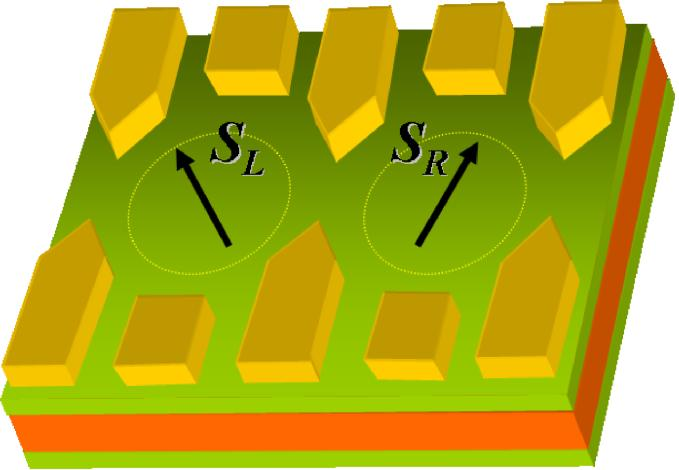
\includegraphics[width=0.75\linewidth]{img/QD.png}
    \caption{Ein doppel Quantum-Dot Qubit}
    \label{fig:double-Quantum-Dot}
\end{figure}

In der Abbildung ist ein Doppel Quantum-Dot Qubit dargestellt. Sowohl in $S_L$ als auch $S_R$ befinden sich Elektornen. Beide können seperat voneinander, sowohl im Spin als auch Ladung, manipuliert werden.
Durch die physikalische Nähe der beiden Quantum-Dots können durch Tunnelkopplung und Austauschwechselwirkung die beiden Qubits miteinander verschränkt werden.\\

Die Umsetzung dieser Methode beschränkt sich hauptsächlich auf die Spin-Variante. Der Grund dafür ist, dass durch die hohe Ladungsanforderung der Ladungsvariante die Qubits sehr empfindlich gegenüber Störungen sind.
Außerdem sind die Nachteile der Spin-Variante gegenüber der Ladungsvariante nicht so gravierend.\\
Jedoch sind die größten Herausforderungen die Herstellung der Halbleiterstrukturen und die Kontrolle der Elektronen in den Quantum-Dots.
Damit ist der größte Vorteil, die hohe Skalierbarkeit, auch der größte Nachteil, da die Herstellung und Kontrolle von vielen Quantum-Dots sehr aufwendig und schwierig ist.\\

\subsubsection{Topologische Quantencomputer}
\label{subsub:topologische_quantencomputer}
Der Ansatz von topologischen Quantencomputern ist völlig anders als die bisher genannten. Im Gegensatz zu verher erläuterten Quantencomputern, welche auf Eigenschaften einzelner Elektronen oder Energieniveaus basieren, basieren topologische Quantencomputer auf topologischen Eigenschaften von Materie.\\
Diese Methode soll das Problem der Dekoheränz minimieren, indem sie Qubits aus Majorana-Partikeln aufbauen.\\

\textbf{Topologie in der Physik}\\
In einem physikalischem System beschreibt die Topologie die Eigenschaften, welche sich nicht durch Deformation verändern lassen.
Ein Beispiel hierfür ist ein Kaffeebecher, der sich durch Verformung in eine Donutform umwandeln lässt. Beide haben die topologische Eigenschaft eines Loches.
Daraus folgernd ist es nicht möglich, einen Kaffeebecher oder ein Donut in eine Kugel zu verformen ohne die topologische Eigenschaft zu verändern.\\

\textbf{Funktionsweise}\\
Die physikalische Grundlage für topologische Quantencomputer liegt in speziellen Materialien und Systemen, die topologische Materiephasen unterstützen.
Ein prominentes Beispiel ist die Verwendung von Majorana-Quasiteilchen, die in bestimmten Supraleitern auftreten können.\\

\begin{figure}[H]
    \centering
    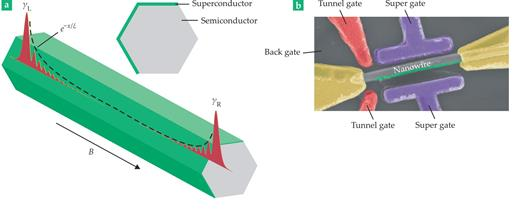
\includegraphics[width=0.75\linewidth]{img/Majorana.png}
    \caption{Nanowire mit Majorana-Quasiteilchen}
    \label{fig:Majorana}
\end{figure}

In der Abbildung ist ein Nanowire dargestellt, der durch ein Supraleiter und ein Magnetfeld in eine topologische Phase gebracht wird.
Diese Art von Partikel treten immer als Paar auf und bilden eine Art Brücke zwischen den Enden des Nanowire und besteht auf einer Vielzahl von Elektronen.
Diese Brücke wird durch die topologischen Eigenschaften der Majorana-Partikel stabilisiert und ist somit weniger anfällig gegenüber Störungen.\\


\begin{tcolorbox}[title=Kommentar,
    title filled=false,
    colback=cyan!5!white,
    colframe=cyan!75!black]
    Die Vertiefung der durch den Quanten-Hall Effekt entsteht wird nur oberflächlich behandelt. Ist jedoch essentiell für die Funktionsweise von Topologischen Quantencomputern.
\end{tcolorbox}

\textbf{Verpflechtung}\\
Braiding ist der Prozess, bei dem die Majorana-Partikel miteinander verflochten werden, um die Quantenbits zu manipulieren. 
Dies passiert auf einer zweidimensionalen Oberfläche, auf der die Majorana-Partikel miteinander verflochten werden.\\

\begin{figure}[H]
    \centering
    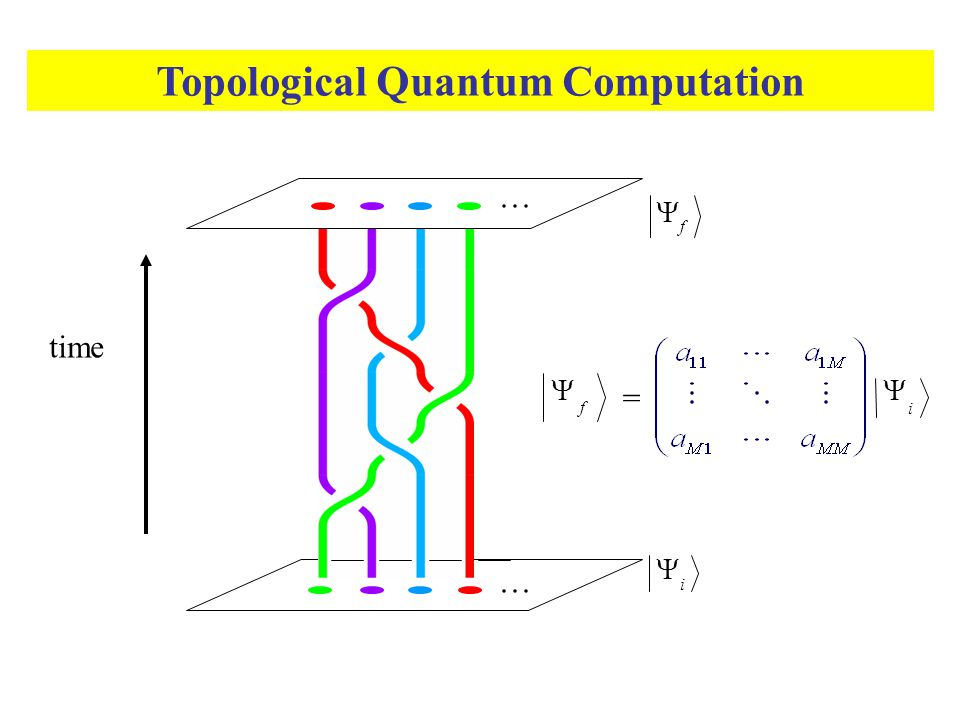
\includegraphics[width=0.75\linewidth]{img/TQC.png}
    \caption{Braiding von Majorana-Quasiteilchen}
    \label{fig:Braiding}
\end{figure}

Hierbei ist die Reihenfolge sehr wichtig, da durch diese Reihenfolge Quantenoperationen realisiert werden.
Jede Verpflechtung entspricht einer Quantenoperation und durch die Kombination von mehreren Verpflechtungen können beliebige Quantenoperationen realisiert werden.\\

Da die Informationen und Quantenoperationen in der Topologie steckt, sind sie gegenüber kleinen Fehlern in der Bewegung/Störungen unempfindlich.\\

\begin{tcolorbox}[title=Kommentar,
    title filled=false,
    colback=cyan!5!white,
    colframe=cyan!75!black]
    Die Technische Umsetzung von topologischen Quantencomputern ist deutlich komplizierter als es in diesem Abschnitt oberflächlich beschrieben ist.\\
    Bisher hat nur Google einen topologischen Quantencomputer vorgestellt, der jedoch noch nicht in der Lage ist, Quantenoperationen durchzuführen.
\end{tcolorbox}

\subsection{Quantum Error Correction}
\label{sub:quantum_error_correction}
Quantum Error Correction, oder auch QEC genannt, ist grundlegend wichtig für die funktionellen Betrieb eines Quantencomputers. Wie bereits in den vorherigen Abschnitten beschrieben,
sind Qubits sehr anfällig gegenüber Dekoheränz und Quantenrauschen.\\

\textbf{Warum ist Fehlerkorrektur notwendig}\\
Es ist unabdingbar, dass eine Fehlerkorrektur in Quantencomputern implementiert wird, da die Fehleranfälligkeit von physischen Qubits durch bessere Herstellung nur einen gewissen Grad an Fehlertoleranz aufbringen kann, welche nicht genug ist.\\

Fehler treten in Quantencomputer durch drei Hauptquellen auf.\\
1. \textbf{Dekoheränz:} Äußere Einflüsse wie Temperaturschwankungen oder elektromagnetische Felder zerstören die koheränten Eigenschaften der Qubits.\\
2. \textbf{Phasen-Flip-Fehler:} Die Phasenwinkel zwischen den Quantenzuständen werden verändert($\ket{0}\rightarrow\ket{0},\ket{1}\rightarrow-\ket{1}$).\\ 
3. \textbf{Bit-Flip-Fehler:} Die Zustände der Qubits werden verändert ($\ket{0}\rightarrow\ket{1},\ket{1}\rightarrow\ket{0}$).\\

Bei der Fehlerkorrektur von Quantencomputern ist jedoch zu beachten, dass diese nicht wie bei herkömmlichen Computern da durch das No-Cloning-Theorem keine Quanteninformationen kopiert werden können.\\

\textbf{Grundprinzip}\\
Quanten-Fehlerkorrektur verwendet \textbf{Redundanz} um Fehler zu detektieren und zu korrigieren, ohne das die eigentliche Quanteninformationen direkt ausgelesen werden.\\

Eine Art der Redundanz ist der Steane-Code, welcher auf 7 Qubits basiert. Dieser Zusammenschluss aus 7 Physischen Qubits bildet ein logisches Qubit,
welches maximal einen Fehler auf einem der 7 Qubits korrigieren kann. Treten jedoch mehrere Fehler auf, kann der Steane-Code diese nicht mehr korrigieren.\\

\begin{figure}[H]
    \centering
    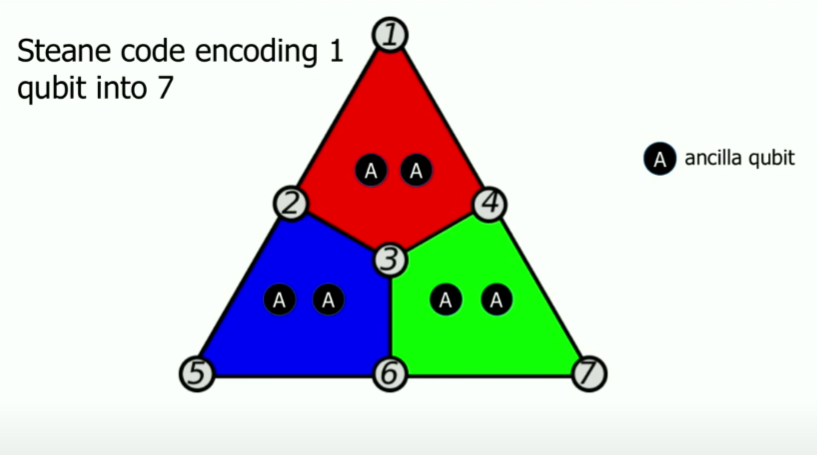
\includegraphics[width=0.75\linewidth]{img/Steane.png}
    \caption{Steane-Code}
    \label{fig:Steane}
\end{figure}

Um die Qubits zu überwachen werden zusätzliche Qubits benötigt, da das direkte Auslesen der daten Qubits den Quantenzustand zerstören würde.
Diese zusätzlichen Qubits werden als \textbf{Ancilla Qubit} bezeichnet und mit den eigentlichen Qubits verschränkt.\\

\textbf{Fehlertoleranz}\\
Diese Herangehensweise ist jedoch auch nicht perfekt. Die Ancilla Qubits sind gleichermaßen anfällig gegenüber Fehlern wie die eigentlichen Qubits.\\

\begin{figure}[H]
    \centering
    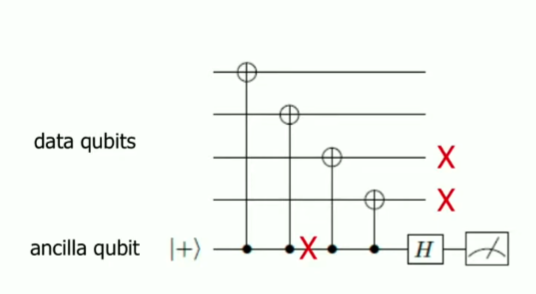
\includegraphics[width=0.75\linewidth]{img/Fehlertoleranz.png}
    \caption{Fehlertoleranz von Ancilla Qubits}
    \label{fig:Fehlertoleranz}
\end{figure}

Dieses Abbildung zeigt, wie ein einzelner Fehler in einem CNOT Gatter auf dem Ancilla Qubit Messung der Daten Qubits als Fehler kennzeichnet, obwohl diese nicht fehlerhaft sind.\\
Die Folge hieraus ist, dass die Fehlerkorrektur mit wenigen Qubits nicht ausreicht um diesen logischen Qubit vollkommen fehlerfrei zu halten.\\

Hierbei werden zwischen zwei Paritätchecks unterschieden. Ein $Z$ und $X$ Parität, welcher festlegt, ob der Fehler in den Ancilla Qubits CNOT Gattern oder den Daten Qubits aufgetreten ist.\\

\textbf{Suface Code}\\
Eine weitere Methode zur Fehlerkorrektur ist der Surface Code, welcher auf einem 2D Gitter von Qubits basiert.
Dieser Code ist in der Lage Fehler zu detektieren und zu korrigieren, solange die Fehlerdichte unter einem bestimmten Wert bleibt.\\

Die Größe des Surface Codes ist variabel und kann skaliert werden, um die Fehlerkorrektur zu verbessern.
Es gibt jedoch ein Threshold, an der die Vergößerung des Codes keine Verbesserung mehr bringt.
Durch die vorher besprochene Fehlertoleranz der Ancilla Qubits wird die Effektivität des Surface Codes gedeckelt.
Die Fehler in der Korrektur werden hierbei mehr, als wenn keine Korrektur vorgenommen wird und es würde keinen Sinn ergeben, den Surface Code weiter zu vergößern.\\

Die Nachfolgende Abbildung eines Surface Codes des Grades $d=3$ zeigt wie die Qubits in einem 2D Gitter angeordnet sind und wie die Fehlerkorrektur durchgeführt wird.
Jede Überschneidung des Gatters stellt ein physischen Qubit dar. Die Kreise in den Quadraten sind die Ancilla Qubits, welche die Fehlerkorrektur durchführen.\\

\begin{figure}[H]
    \centering
    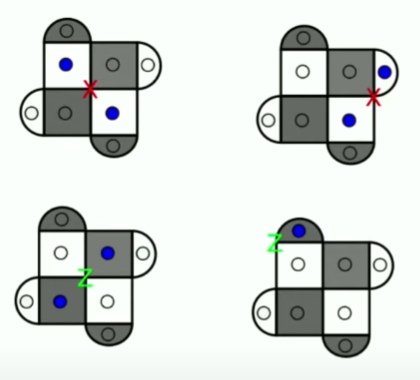
\includegraphics[width=0.6\linewidth]{img/Errors.png}
    \caption{Fehlerkorrektur durch Surface Code des Grades $d=3$}
    \label{fig:Surface-Code}
\end{figure}

Ancilla Qubits in einem weißen Feld prüfen die Qubits auf ein logisches $X$ und Ancilla Qubits in einem Schwarzen Feld prüfen die Qubits auf ein logisches $Z$.\\

Ancilla Qubits, die ein Fehler erkennen, werden als Blau markiert. Durch die Position dieser und für welche Daten Qubits diese zuständig sind wissen wir welche Qubits fehlerhaft sind.\\

\textbf{Praktische Umsetzung}\\
Am 09.12.2024 hat Google den ersten selbst korrigierenden Quantencomputer vorgestellt, der auf dem Surface Code basiert.
Der Chip namens \textbf{Willow} basiert auf 105 physischen Qubits, wobei diese auf der 7x7 Surface Code Architektur aufbaut.
Dies resultiert in 49 Qubits, die deutlich weniger anfällig gegen Fehler sind als phyische Qubits. Die restlichen Qubits werden für Parität und error Korrektur gebraucht.\\

\begin{figure}[H]
    \centering
    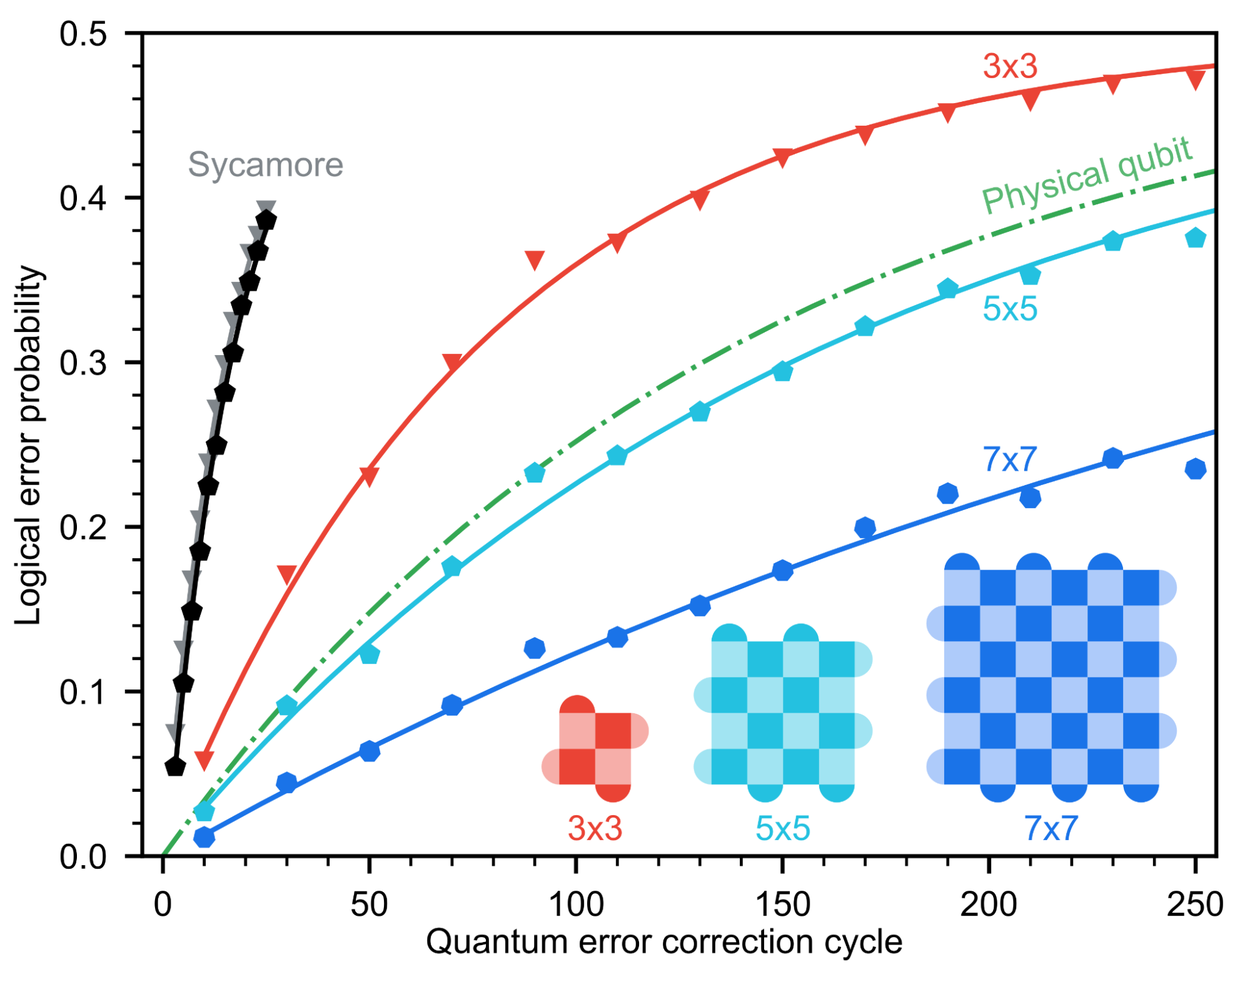
\includegraphics[width=0.7\linewidth]{img/Surface-Code-Scaling.png}
    \caption{Error Korrektur des 7x7 Surface Code}
    \label{fig:Willow}
\end{figure}

Außerdem wurde durch die Anwendung des Surface Codes die $T_1$ Zeit von $20\mu s$ auf $68\mu s\pm13\mu s$ erhöht und ermöglich hierdurch mehr Operationen pro Qubit.\\
% \include{content/chsh}
\section{Schluss}
\label{sec:schluss}

Zusammenfassend lässt sich festhalten, dass die Quanteninformatik ein vielversprechendes Feld darstellt, dass das Potenzial hat, klassische Computer in zahlreichen Bereichen zu übertreffen.
So haben wir in den Grundlagen die fundamentalen Prinzipien und Funktionsweisen für Quantencomputer herausgestellt.
Mit Quantenbits ist es möglich, mehrere Zustände gleichzeitig zu repräsentieren, was zusammen mit der Zerstörung der Superposition durch Messungen einen entscheidenden Vorteil in der Kryptografie bietet.
Die Verschränkung ermöglicht es, dass zwei Quantenbits in einem Zustand sind, sodass die Messung eines Bits den Zustand des anderen beeinflusst, was die Grundlage für Quantenteleportation bildet.\\

Mit dem No Cloning Theorem haben wir eine der grundlegendsten Einschränkungen und gleichzeitig auch Möglichkeit in der Quanteninformatik kennengelernt.
Es besagt, dass ein unbekannter Quantenzustand nicht kopiert werden kann.
Zum einen erfordert dies eine neue Denkweise bei der Entwicklung von Algorithmen, zum anderen bietet es die Möglichkeit, Quantenkommunikation abhörsicher zu gestalten.\\

Die Quantenteleportation ist eines der faszinierendsten Konzepte der Quanteninformatik, welches die Übertragung von Informationen ohne physische Bewegung ermöglicht.
Hier liegt die Herausforderung in der Erzeugung und Aufrechterhaltung der Quantenverschränkung, sowie der Notwendigkeit der klassischen Kommunikation.\\

Eine der größten technischen Hürden bildet die Dekohärenz, die durch die Wechselwirkung der Quantenbits mit ihrer Umgebung entsteht.
Es wurde beleuchtet, wie sie entsteht und berechnet wird, sowie wie sie durch Fehlerkorrekturverfahren minimiert werden kann.
Außerdem wurden unterschiedliche Modelle für universelle Quantencomputer vorgestellt, die auf verschiedenen Technologien basieren.\\

Jedoch haben wir auch gesehen, dass Quantencomputer nicht nur eine Theorie ist und bereits in der Praxis eingesetzt wird.
So haben wir die Bell-Ungleichung betrachtet und gezeigt, wie sie mit einem Quantencomputer simuliert werden kann.\\

Zusammenfassend lässt sich sagen, dass die Quanteninformatik sowohl ein enormes Potenzial als auch einige fundamentale Herausforderungen birgt.
Die Entwicklung von Quantencomputern und -algorithmen ist ein aktives Forschungsfeld, das in den nächsten Jahren weiter an Bedeutung gewinnen wird.
Wir sind sehr gespannt, wie sich die Technologie entwickeln wird und in welchen Bereichen wir selbst damit auch in Berührung kommen werden.












\bibliographystyle{apalike}
\bibliography{references} % expects file "references.bib"

\end{document}
